% Blue Jay Night Ride: scenario methodology and simulator contract (explanatory companion)
% Build with ./build.sh (XeLaTeX). Figures come from make_figures.py.
\documentclass[11pt,letterpaper]{article}

% ------------------------------------------------------------------ layout
\usepackage[letterpaper,left=1.1in,right=1.1in,top=1in,bottom=1in,headsep=0.3in,footskip=0.45in]{geometry}
\usepackage{fontspec}
\usepackage{unicode-math}
\IfFontExistsTF{Charter}{%
  \setmainfont{Charter}%
  \setmathfont{STIX Two Math}%
}{%
  \setmainfont{Latin Modern Roman}%
  \setmathfont{Latin Modern Math}%
}
\IfFontExistsTF{Helvetica Neue}{\setsansfont{Helvetica Neue}}{\setsansfont{Latin Modern Sans}}
\IfFontExistsTF{Menlo}{\setmonofont[Scale=0.82,HyphenChar=None]{Menlo}}{\setmonofont[HyphenChar=None]{Latin Modern Mono}}

\usepackage{xcolor}
\usepackage{graphicx}
\usepackage{booktabs}
\usepackage{array}
\usepackage{tabularx}
\usepackage{longtable}
\usepackage{enumitem}
\usepackage{float}
\usepackage[font=small,labelfont={bf,sf},format=plain,justification=justified,singlelinecheck=false,skip=6pt]{caption}
\usepackage{framed}
\usepackage{titlesec}
\usepackage{titleps}
\usepackage{microtype}
\usepackage{amsmath}
\usepackage[hidelinks,pdfusetitle]{hyperref}
\usepackage{bookmark}
\usepackage[nameinlink,capitalise]{cleveref}

\hypersetup{
  pdftitle={Building the simulated Night Ride evening: scenario methodology and simulator contract},
  pdfauthor={Team FourSight (EN.553.602, Fall 2026)},
  pdfsubject={Explanatory companion to the scenario methodology, scenario specification and model design},
}

% ------------------------------------------------------------------ colours
\definecolor{ink}{HTML}{1F2933}
\definecolor{muted}{HTML}{5B6370}
\definecolor{rulegrey}{HTML}{D1D5DB}
\definecolor{shade}{HTML}{F4F6F8}
\definecolor{cAssumed}{HTML}{3B6FB6}
\definecolor{cDesigned}{HTML}{C2410C}
\definecolor{cSim}{HTML}{7B3FB6}
\definecolor{cEvid}{HTML}{6B7280}
\definecolor{cDerived}{HTML}{0F766E}
\definecolor{cAccepted}{HTML}{15803D}
\definecolor{cProvisional}{HTML}{A16207}
\definecolor{cProposed}{HTML}{B91C1C}
\definecolor{cOpen}{HTML}{7F1D1D}
\definecolor{heading}{HTML}{0B2545}
\color{ink}

% ------------------------------------------------------------------ paragraphs and lists
\setlength{\parindent}{0pt}
\setlength{\parskip}{0.55em plus 0.15em}
\setlist{itemsep=0.15em,topsep=0.25em,parsep=0.1em,leftmargin=1.4em}
\linespread{1.06}
\renewcommand{\arraystretch}{1.18}
\setlength{\emergencystretch}{2em}
\raggedbottom
\clubpenalty=10000
\widowpenalty=10000

% ------------------------------------------------------------------ headings
\titleformat{\section}{\sffamily\Large\bfseries\color{heading}}{\thesection}{0.6em}{}
\titleformat{\subsection}{\sffamily\large\bfseries\color{heading}}{\thesubsection}{0.6em}{}
\titleformat{\subsubsection}{\sffamily\normalsize\bfseries\color{heading}}{\thesubsubsection}{0.6em}{}
\titlespacing*{\section}{0pt}{1.4em}{0.5em}
\titlespacing*{\subsection}{0pt}{1.1em}{0.35em}
\titlespacing*{\subsubsection}{0pt}{0.9em}{0.25em}

\newpagestyle{main}{%
  \setheadrule{0pt}%
  \sethead{}{}{\sffamily\footnotesize\color{muted}Scenario methodology and simulator contract \textbar{} companion v1.0}%
  \setfoot{}{\sffamily\small\thepage}{}%
}
\pagestyle{main}

% ------------------------------------------------------------------ markers
% Statement kinds (filled) and approval status (outlined)
\newcommand{\marker}[2]{{\setlength{\fboxsep}{1.4pt}\colorbox{#1}{\textcolor{white}{\sffamily\bfseries\scriptsize\strut #2}}}}
\newcommand{\Assumed}{\marker{cAssumed}{ASSUMED}}
\newcommand{\Designed}{\marker{cDesigned}{DESIGNED CHECK}}
\newcommand{\Simulated}{\marker{cSim}{SIMULATED}}
\newcommand{\Evidence}{\marker{cEvid}{APRIL EVIDENCE}}
\newcommand{\Derived}{\marker{cDerived}{DERIVED}}
\newcommand{\status}[2]{{\setlength{\fboxsep}{1.1pt}\fcolorbox{#1}{white}{\textcolor{#1}{\sffamily\scriptsize\strut #2}}}}
\newcommand{\Accepted}{\status{cAccepted}{accepted}}
\newcommand{\Provisional}{\status{cProvisional}{provisional}}
\newcommand{\Proposed}{\status{cProposed}{proposed, not approved}}
\newcommand{\Open}{\status{cOpen}{open}}
\newcommand{\Correction}{\status{cAccepted}{correction}}

% state names, file names, decision IDs
\DeclareRobustCommand{\st}[1]{\texttt{\detokenize{#1}}}
\DeclareRobustCommand{\fn}[1]{\texttt{\detokenize{#1}}}
\newcommand{\D}[1]{D-#1}

% shaded call-out
\newenvironment{callout}[1][]{%
  \def\FrameCommand{\fboxsep=8pt\colorbox{shade}}%
  \MakeFramed{\advance\hsize-\width\FrameRestore}%
  \ifx\relax#1\relax\else{\sffamily\bfseries\color{heading}#1}\par\smallskip\fi}%
  {\endMakeFramed}

% a block card: evidence -> calculation/assumption -> input -> limitation -> sensitivity
\newenvironment{blockcard}{%
  \par\smallskip\noindent
  \tabularx{\textwidth}{@{}>{\raggedright\arraybackslash\sffamily\small\bfseries\leavevmode\color{heading}}p{2.55cm}>{\raggedright\arraybackslash}X@{}}
  \toprule}{%
  \bottomrule\endtabularx\par\medskip}
\newcommand{\cardrow}[2]{#1 & #2 \\ \addlinespace[2pt]}

\newcolumntype{L}{>{\raggedright\arraybackslash}X}
\newcolumntype{P}[1]{>{\raggedright\arraybackslash}p{#1}}

\begin{document}

% ================================================================== title page
\begin{titlepage}
\thispagestyle{empty}
\vspace*{0.6in}
{\sffamily\small\color{muted} Blue Jay Night Ride optimization \textbar{} Team FourSight \textbar{} EN.553.402/602, Fall 2026\par}
\vspace{0.25in}
{\sffamily\fontsize{24}{29}\selectfont\bfseries\color{heading} Building the simulated\\ Night Ride evening\par}
\vspace{0.12in}
{\sffamily\Large\color{heading} Scenario methodology and simulator contract,\\ explained\par}
\vspace{0.35in}
{\large An explanatory companion to the scenario methodology (v1.1), the scenario specification (v0.5) and the model design (v0.3)\par}
\vspace{0.3in}
{\sffamily\small
\begin{tabular}{@{}ll@{}}
Status & Version 1.0 for team review. Section~7 reports the verified M0--M1 status.\\
Date & 22 October 2026\\
Sources read & Versions and fingerprints in \cref{app:sources}\\
\end{tabular}\par}
\vfill
\begin{callout}[What this document is, and is not]
This is a \textbf{reading companion}. It explains how one simulated Night Ride evening is built from April 2026's aggregate dashboard, what the simulator must do, and how the van dispatcher scores its plans. It introduces \textbf{no new rule, number or decision}. Every number is quoted from the documents listed in \cref{app:sources}; where they disagree, the decision log wins, then the scenario specification. Points where the sources disagreed while this companion was written, and how the authoritative documents settled them, are listed in \cref{app:gaps}.

Only Section~7 reports simulated outcomes, and only from designed validation cases (levels L1--L4). No Lyft-rule comparison has been run, and nothing here says any rule is better. Everywhere else, outcomes are design statements or hand-computed checks.
\end{callout}
\end{titlepage}

% ================================================================== reading guide
\section*{How to read this document}
\addcontentsline{toc}{section}{How to read this document}

Sections 1 to 6 are meant to be read in order. Section~1 states the question and the boundaries of the system. Section~2 explains what April's aggregate data can and cannot tell us. Section~3 builds a scenario one block at a time. Section~4 restates the simulator's rules in plain words, Section~5 explains the dispatcher's mathematics, and Section~6 follows one request from start to finish. The appendices hold the decision history, the symbols, the open points and the references.

Three kinds of statement are easy to confuse in a simulation study, so every important statement carries a marker:

\begin{center}
\small
\begin{tabularx}{\textwidth}{@{}p{3.5cm}L@{}}
\toprule
\textbf{Marker} & \textbf{Meaning}\\
\midrule
\Assumed & An input rule or behaviour that \emph{we chose}. It is not a measured Hopkins fact. Example: riders' patience follows a placeholder distribution.\\
\Designed & A small validation case built by hand (levels L1--L4) whose correct answer is known in advance. It checks the machinery, not the research question.\\
\Simulated & An outcome that \emph{only the simulation produces}: waits, cancellations, no-shows, transfers, completions. In this document such outcomes appear only in Section~7, from a designed validation case.\\
\Evidence & A number read from April 2026's aggregate dashboard, as quoted in the source documents.\\
\Derived & Arithmetic on April numbers (for example a ratio), resting on stated assumptions.\\
\bottomrule
\end{tabularx}
\end{center}

Decisions also carry an \textbf{approval status}, because several 21 October conventions are proposals rather than team approvals:

\begin{center}
\small
\begin{tabularx}{\textwidth}{@{}p{3.5cm}L@{}}
\toprule
\Accepted & The team decided it (or it corrects a demonstrable error).\\
\Provisional & A working value or choice that may change, usually after calibration or a benchmark.\\
\Proposed & Written down by the consolidation review of 21 October but not separately approved by the team.\\
\Open & No decision yet.\\
\bottomrule
\end{tabularx}
\end{center}

Decision identifiers such as \D{36} refer to rows of the project decision log (\cref{app:decisions}). File names such as \fn{scenario_spec.md} refer to the repository's \fn{docs/technical/} folder.

\clearpage
\tableofcontents
\listoffigures
\listoftables
\clearpage

% ================================================================== 1
\section{The research question and the boundaries of the system}\label{sec:question}
This section states what the study asks, what is held fixed, and where the modelled system ends.

\subsection{The question}
Johns Hopkins' Blue Jay Night Ride is an on-demand, shared van service. When the vans fall behind, a human dispatcher can send a waiting rider a Lyft instead. The study asks:

\begin{callout}
Holding the van dispatcher fixed, which dispatcher-initiated Lyft transfer rule gives Homewood riders the best outcomes for the resources it uses (Lyft bookings and van-kilometres)?
\end{callout}

The wording follows the team's primary question (\D{26}), refined to \emph{resource use} rather than cost because no money is modelled (\D{45}). The study is about \textbf{policy}, the Lyft rule, not about which algorithm is cleverest. Every rule is run on the same simulated evenings, one rule at a time, with everything else held fixed (\D{28}).

\subsection{Three things kept apart}
A fair comparison needs a clean separation between what goes in, what we vary, and what comes out (\cref{tab:three}). Inputs are identical for every rule; the rule is the only thing that changes; outcomes are produced only by the simulation, never typed in.

\begin{table}[!htbp]
\centering\small
\caption{Inputs, policies and outcomes are kept apart (after the specification §1 and the methodology §3).}\label{tab:three}
\begin{tabularx}{\textwidth}{@{}P{2.3cm}LP{3.6cm}@{}}
\toprule
\textbf{Kind} & \textbf{Examples} & \textbf{Who sees it}\\
\midrule
Inputs (public) & Request time, origin, destination, party size; vans on duty & The dispatcher, but only once a request has arrived\\
Inputs (hidden) & Patience deadline, presence draw, consent draw, Lyft delay & Only the simulator, and only when the relevant event happens\\
Policy & Dispatcher, objective weights, re-planning cadence, Lyft rule, dispatcher lag & Fixed for a run\\
Outcomes \Simulated & Actual waits, pickups, cancellations, no-shows, transfers, Lyft completions, van-km & Evaluation only\\
\bottomrule
\end{tabularx}
\end{table}

\begin{figure}[!htbp]
\centering
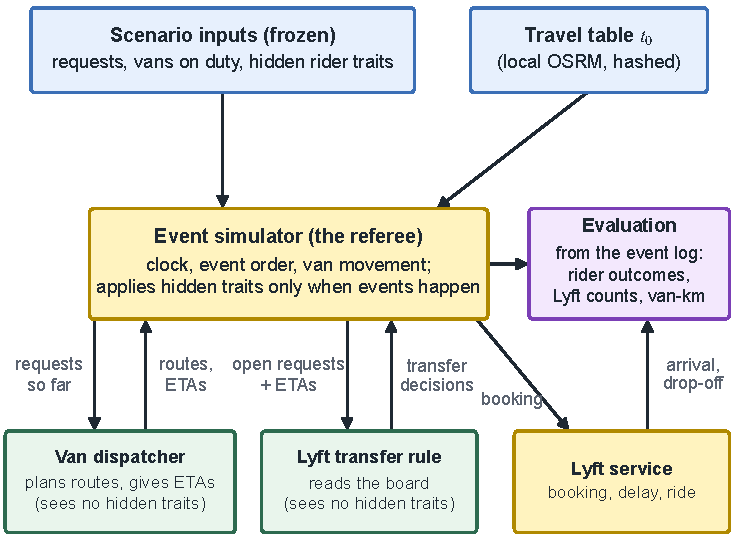
\includegraphics[width=\textwidth]{figures/f1_system.pdf}
\caption[The system in one picture]{The system in one picture. The frozen scenario and the travel table feed the event simulator, which acts as referee: it owns the clock and applies each rider's hidden traits only when the relevant event happens. The van dispatcher and the Lyft transfer rule (green) are policies; they see only what a real dispatcher could see. The Lyft service is deliberately thin: the study needs \emph{when} a transferred rider is picked up, not how Lyft matches drivers. After \fn{scenario_methodology.md} §2.}\label{fig:system}
\end{figure}

\subsection{System boundaries}
The boundaries below are fixed for the main experiments. Each has a decision behind it. \Cref{fig:system} shows how the parts fit together.

\begin{itemize}
\item \textbf{Area:} Homewood Night Ride \emph{including the Peabody area}, as April was operated (\D{27}) \Accepted. East Baltimore demand, policies and targets are excluded (\D{23}) \Accepted.
\item \textbf{Door-to-door service, no stop experiment:} riders are picked up at a snapped curb point near their location. The digitized April hotspots are \emph{demand-generation points}, not stops; stop consolidation is out of scope (\D{24}) \Accepted.
\item \textbf{When requests arrive:} 18:00--21:00, the busiest three hours, beginning at the first hour of service so no backlog is inherited (design trail §1) \Accepted. After 21:00 no new requests arrive, and the run continues until every accepted request is resolved (the closing rule, \D{36}; build convention \D{46}(6) \Proposed).
\item \textbf{Fleet:} five vans with 14 seats each, on duty throughout 18:00--21:00 and then until the backlog is finished (\D{36}) \Accepted. The benefit of a sixth van is measured on the \emph{same} requests (\D{37}) \Accepted.
\item \textbf{Parties of five:} a party of five that is transferred travels together as \emph{one} Lyft XL booking; parties of one to four use a standard Lyft (\D{33}). This is an accepted modelling instruction based on user-supplied operational knowledge, not verified Hopkins policy.
\item \textbf{No money:} the model has no fares, fees or dollar expenditure, and unknown prices are not set to zero. Resource use is reported as counts: transfer decisions, bookings, completed Lyft trips (standard and XL separately), van-km (\D{45}) \Accepted.
\item \textbf{Service quality is not safety:} shorter outdoor waits at night are a service-quality proxy for the program's safety purpose. The model measures waits, cancellations and ride times, not physical safety (\fn{model_design.md} §4.4).
\item \textbf{Targets as reporting thresholds:} 15-minute pickup, 20-minute ride and 20-minute busy-time arrival, taken from the JHU page wording captured around April 2026. The live page read on 21 October 2026 states 20/25/25. The two readings are kept distinct, and neither is treated as proof of operating policy (\D{49}).
\end{itemize}

\subsection{How results will be judged (pointer)}
The rules for judging results live in the draft pre-registration (\fn{preregistration_v2.md}), which is frozen when the first main (L6) comparison run starts. In outline:
\begin{itemize}
\item Rules are compared on \textbf{paired} nights (the same 30 evenings for every rule), and the answer is a \textbf{frontier} of rider outcome against resource use, not a single winner. ``Send everyone to Lyft'' is one end of that frontier, never the answer.
\item The proposed primary rider outcome is the share of \emph{all} requests not reached by a vehicle (van or Lyft) within 15 minutes, counting riders who cancelled as not reached (\D{50}(2) \Proposed). Wait percentiles among picked-up riders leave out those who gave up, so they are read beside it.
\item Comparisons use non-inferiority margins rather than ``the confidence interval contains zero''. The correction of that wording is \Accepted{}; the margins themselves (1 minute for wait percentiles, 2 percentage points for shares) are \Proposed{} (\D{50}).
\end{itemize}

% ================================================================== 2
\section{What April's aggregate evidence identifies, and what it leaves unknown}\label{sec:evidence}
This section separates what the April data can support from what has to be assumed. It explains why the study builds a family of plausible evenings rather than one reconstructed night.

\subsection{What the dashboard gives}
The only operational source is the April 2026 TransLoc dashboard for the Homewood Night Ride. It is restricted, so this document uses only the aggregate numbers already quoted in the project's documents. It gives \textbf{totals and shares}: requests by status, completed rides by hour, average vehicles by hour, origin and destination density maps with printed bubble counts, and a few wait and ride percentiles. \Cref{tab:april} lists the numbers this document relies on.

\begin{table}[!htbp]
\centering\small
\caption[April 2026 aggregates used in this document]{April 2026 aggregates used in this document, as quoted in the sources. All are \Evidence{} except the last block, which is \Derived{} under stated assumptions.}\label{tab:april}
\begin{tabularx}{\textwidth}{@{}LP{3.6cm}P{3.3cm}@{}}
\toprule
\textbf{Quantity} & \textbf{Value} & \textbf{Where quoted}\\
\midrule
Recorded requests (Completed + Canceled + No Show; Denied read as 0) & 50,297 & spec §3.2\\
Completed rides & 24,095 & spec §3.2\\
``No Show'' & 2,359 (4.7\% of all requests; 2.8--6.4\% by day) & trail §8\\
``Canceled'' & $\approx$ 47\% of requests (31--68\% by day) & spec §12\\
Passengers per completed booking & 1.386 & corrections, 21 Oct\\
Lyft share of riders & $\approx$ 24.5\% (10--46\% by day) & spec §12\\
Completed-ride wait & median $\sim$10--13 min; P90 $\sim$17--21 min & spec §12\\
Ride time P90 & $\sim$24 min & spec §12; model §4.3\\
Completed rides per van-hour & $\approx$ 5.1 (6.2 at 6 pm) & spec §12\\
``All services'' vehicles at 6 pm & $\approx$ 27.6, tapering later; averaged over 29 days & methodology §4; \D{49}\\
\midrule
Requests per completed ride $R/C$ & 50,297 / 24,095 = 2.087 \Derived & methodology App.~B\\
Load per van $\rho_h$, 18/19/20 h & 12.85 / 10.10 / 10.71 \Derived & spec §3.2\\
\bottomrule
\end{tabularx}
\end{table}

\subsection{Why aggregates cannot pin down one scenario}
The dashboard never shows one rider's request, wait and outcome together. That has three consequences, each of which shapes the design (\fn{scenario_methodology.md} §5).

\textbf{1. Many different nights produce the same totals.} The maps give how many trips start in each zone and how many end in each zone, but not which start goes with which end. A toy example makes the point (\cref{tab:toy}): two very different trip tables have exactly the same row and column totals. The same is true of hourly counts, which fit many within-hour patterns. So the design picks one principled member (maximum-entropy pairing; uniform times within the hour) and tests deliberately stressed alternatives (burst, far-trip, dispersed geography). It never claims to be \emph{the} April night.

\begin{table}[!htbp]
\centering\small
\caption[Toy example: one set of margins, two trip tables]{Toy example (not project data). Both tables have origins X~=~3, Y~=~2 and destinations X~=~2, Y~=~3, yet they describe different travel patterns.}\label{tab:toy}
\begin{tabular}{@{}lccc@{\hspace{3em}}lccc@{}}
\toprule
\multicolumn{4}{c}{Table one} & \multicolumn{4}{c}{Table two}\\
\cmidrule(r{2.5em}){1-4}\cmidrule{5-8}
from \textbackslash{} to & X & Y & total & from \textbackslash{} to & X & Y & total\\
\midrule
X & 1 & 2 & 3 & X & 0 & 3 & 3\\
Y & 1 & 1 & 2 & Y & 2 & 0 & 2\\
total & 2 & 3 & 5 & total & 2 & 3 & 5\\
\bottomrule
\end{tabular}
\end{table}

\textbf{2. Behaviour is confounded with operations.} A long wait followed by ``Canceled'' could be an impatient rider, or a dispatcher who handed the rider to Lyft (which is likely recorded as ``Canceled''). The totals cannot separate the two. That is why the rider share of ``Canceled'' is carried as a 50--75\% \emph{range} (\D{39}), and why patience will be calibrated to a \emph{set} of acceptable values rather than one.

\textbf{3. Shares do not say who.} ``4.7\% of requests were no-shows'' does not say which riders, or whether presence depends on how long they waited. A per-arrival no-show probability follows from the totals only under a stated mapping of dashboard statuses (\cref{sec:noshow}).

\begin{callout}[What the study can and cannot claim]
The claim is conditional: \emph{in scenarios consistent with April's aggregates, rule X does better than rule Y, and this holds across the identified set and the stress patterns.} The study cannot claim that rule X would have done better on any particular April night.
\end{callout}

\subsection{Calibration keeps a set, not a point}
Before any comparison, the base pattern of the full-night level is to be calibrated against dashboard-comparable bands: completed share $\approx$ 48\%, ``Canceled'' $\approx$ 47\%, Lyft rider share $\approx$ 24.5\%, no-shows $\approx$ 4.7\% of all requests, completed-ride wait and ride percentiles, and completed rides per van-hour (spec §12). The knobs are the load ratio $\rho$, the patience scale, the travel multiplier and the threshold of the status-quo rule. Every knob setting that passes is kept (the \emph{identified set}), and the main comparison is re-run at its extremes (pre-registration §5). Known limits remain: waits are survivor-biased, the cancellation link is correlational, vehicle counts mix services, there are no hourly Lyft data, and the scaled-down system is less dense than the real one.

% ================================================================== 3
\section{Building a scenario, block by block}\label{sec:blocks}

A \textbf{scenario} is one simulated evening: a list of requests (when each arrives, where it starts and ends, how many riders it carries), the vans on duty, and each request's hidden traits. It is the \emph{same} evening for every rule. A scenario contains inputs only; cancellations, no-shows, transfers and completions are \Simulated{} and never written into it.

Each ingredient has its own seeded random stream (times, places, party sizes, patience, no-shows, consent, Lyft delays, and so on). Changing one ingredient never reshuffles the others, and every rule sees identical riders with identical hidden traits. This is the method of \emph{common random numbers}. Each recipe is turned into 30 nights with 30 seeds (spec §0, §11).

Each block below follows the same pattern: the evidence, the calculation or assumption, the chosen input, its limitation, and the sensitivity that tests it.

\subsection{Volume: how many requests}\label{sec:volume}
The data give the workload per vehicle in April, not the demand a five-van system would face. The design therefore copies April's \emph{load per van}, hour by hour, and gives the scenario's vans that load (\D{35}).

For each clock hour $h$:
\begin{equation}
\rho_h = \frac{C_h}{30}\times\frac{R}{C}\div V_h, \qquad N_h = \rho_h\, v_h ,
\end{equation}
where $C_h$ is April's completed rides in that hour over the month, $R/C = 2.087$ is recorded requests per completed ride, $V_h$ is the average ``All services'' vehicles in that hour, and $v_h$ is the scenario's vans in that hour.

\textbf{Worked example: 168 requests.} With five vans every hour, $5\rho_h$ gives 64.25, 50.50 and 53.55, which sum to 168.3. The \emph{largest-remainder rule} then makes whole numbers that add up to the rounded total:
\begin{enumerate}
\item round the total: 168;
\item floor each hour: 64, 50, 53 (sum 167);
\item give the one leftover unit to the hour with the largest fraction (0.55 for 20:00), so the result is \textbf{64 / 50 / 54 = 168}.
\end{enumerate}
The same rule with April-shaped availability (5, 4.95, 4.46 vans) gives 64 / 50 / 48 = 162; that tapering case is kept for later.

\begin{figure}[!htbp]
\centering
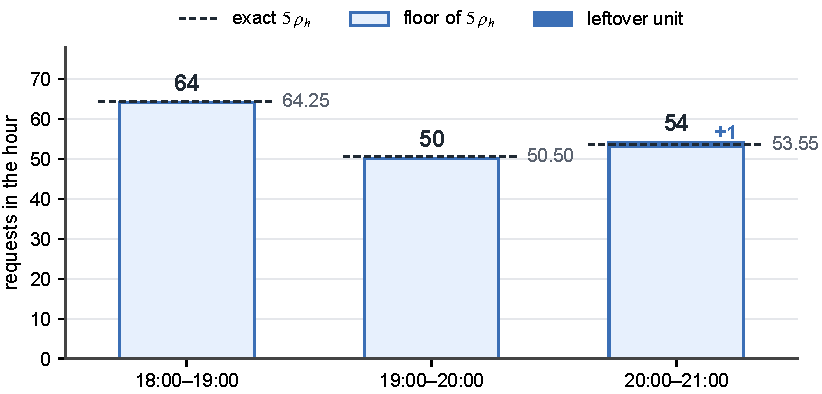
\includegraphics[width=\textwidth]{figures/f2_volume.pdf}
\caption[Largest-remainder rounding of the hourly request counts]{Largest-remainder rounding of the hourly request counts at five constant vans. Dashed lines are the exact values $5\rho_h$; bars are the whole numbers used. The single leftover unit goes to 20:00--21:00, whose fraction (0.55) is the largest.}\label{fig:volume}
\end{figure}

\begin{blockcard}
\cardrow{Evidence}{April status totals (requests 50,297; completed 24,095), completed rides by hour, average vehicles by hour (``All services'') \Evidence.}
\cardrow{Calculation}{$\rho_h$ = 12.85 / 10.10 / 10.71 \Derived; $N_h = \rho_h v_h$ with largest-remainder rounding. Assumes every status is one request with Denied zero, the same request-to-completion ratio in every hour, completed rides counted by request hour, and ``All services'' standing in for Homewood vans \Assumed.}
\cardrow{Chosen input}{64 / 50 / 54 = 168 requests for 18:00--21:00 at five constant vans (\D{36}). The availability choice is \Accepted; the count is \Provisional{} (a derived workload, not measured April demand).}
\cardrow{Limitation}{The vehicle count mixes services and averages 29 days, not 30 ($\pm$3\% on $\rho$). Scaling demand down with the fleet keeps load per van but not density, so pooling chances are lower than in the real system: results hold ``at the scaled system's density''.}
\cardrow{Sensitivity}{Illustrative range $\sim$150--260 (\D{49}), \emph{not} a confidence interval: if Homewood had 20--35\% fewer vehicles than ``All services'' the count rises to $\approx$210--260; $\sim$10\% rebookings would lower it to $\approx$150. The high-load pattern multiplies $\rho$ by 1.3; $\rho$ is the calibration knob.}
\end{blockcard}

\subsection{Hourly timing: when within the hour}
\begin{blockcard}
\cardrow{Evidence}{Only hourly totals; within-hour bunching is not observed \Evidence.}
\cardrow{Assumption}{A fixed count per hour at uniformly random times, which is a Poisson process conditional on its count \Assumed. The hourly chart is read as request hour (\D{49}(5), a transparent base assumption).}
\cardrow{Chosen input}{A named ``times'' stream per level, pattern and night; every rule replays identical times \Accepted.}
\cardrow{Limitation}{Night-to-night variation in volume is removed (April's daily requests varied by about 11\%). If cancellations concentrate at peaks, the true request profile may tilt earlier.}
\cardrow{Sensitivity}{Burst pattern: 40\% of the 18:00--19:00 requests fall inside one 10-minute block. A random-count (Poisson) variant.}
\end{blockcard}

\subsection{Geography: where requests start and end}
\begin{blockcard}
\cardrow{Evidence}{Density maps with printed bubble counts, digitized and georeferenced into 188 hotspot points and 16 zones; the city maps sum to 24,056 origins and 24,057 destinations, matching completed rides (\D{01}) \Evidence.}
\cardrow{Assumption}{Each hotspot stands for nearby addresses and is used as a demand-generation point; vans stop at the snapped road point (one documented exception, 95~m) \Assumed. Requests share the geography of completed rides, since cancelled requests' locations are unobserved.}
\cardrow{Chosen input}{Reference geography: 188 points over Homewood + Peabody (\D{27}). Travel times come from one base table $t_0$ (local OSRM v6.0.0, Maryland extract, hashed in \fn{MANIFEST.json}, \D{31}). Van time $= t_0\, m_v$, Lyft time $= t_0\, m_L$, each multiplier applied once; base $m_v = m_L = 1.2$ \Assumed, calibrated later. Vans start at a depot on the Homewood campus (\D{17}) \Assumed.}
\cardrow{Limitation}{A city-view bubble stands for a whole neighbourhood (the city view is about four times coarser than the campus view), so the reference stacks many requests on one spot and can flatter pooling exactly where long, isolated trips make Lyft attractive.}
\cardrow{Sensitivity}{Dispersed variant \fn{dispersed_v1} (\D{34}): each of the 19 coarse city-view clusters is spread over 6 road satellites within $\sim$400~m, with the same times, cluster-level pairs, parties and traits; its travel table covers 302 points. Its internal consistency is verified; that does not validate 400~m as true pickup locations. Which geography is the L6 base is \Provisional. Radius 250 / 600~m.}
\end{blockcard}

\subsection{Origin--destination pairing}
\begin{blockcard}
\cardrow{Evidence}{Origin totals and destination totals per place, not pairs \Evidence.}
\cardrow{Calculation}{Gravity $\times$ iterative proportional fitting (IPF). A pair starts with weight $w_o\, w_d\, e^{-\beta_{\text{geo}}\, t_{od}/60}$, with $\beta_{\text{geo}} = 0.1$ per minute of driving; pairs under 60~s of driving are excluded. IPF then rescales until every place's totals equal April's (largest error $\sim10^{-10}$) (\D{18}).}
\cardrow{Chosen input}{Pairs drawn from that table \Accepted; $\beta_{\text{geo}}$ \Provisional. $\beta_{\text{geo}}$ is unrelated to the ride weight $\beta = 0.5$ in the dispatcher's objective.}
\cardrow{Limitation}{The true pairing is \emph{not identified}: every $\beta_{\text{geo}}$ reproduces the margins (\cref{tab:toy}). The same geography is used in every hour.}
\cardrow{Sensitivity}{$\beta_{\text{geo}}$ = 0 / 0.1 / 0.2; a campus-outbound direction variant; the far-trip pattern doubles the probability of trips with an end in the Peabody/downtown zones.}
\end{blockcard}

\subsection{Parties: how many riders per booking}
\begin{blockcard}
\cardrow{Evidence}{April's 1.386 van passengers per \emph{completed} booking \Evidence.}
\cardrow{Assumption}{Party size P(1, 2, 3, 4, 5) = 0.73 / 0.18 / 0.055 / 0.025 / 0.01, mean 1.405 \Assumed. The two means are different quantities; the second was chosen near the first.}
\cardrow{Chosen input}{The average-April shape is the base (\D{38}) \Accepted. Costs and metrics are passenger-weighted, with request-weighted versions also reported. A 14-seat van can take a party of five only when five seats are free at that point in its route.}
\cardrow{Limitation}{Only the mean is near the data; the shape is assumed. About 1\% of bookings ($\approx$1.7 per 168-request night) are parties of five: that is \emph{potential} XL demand. How many XL trips occur depends on the rule and is \Simulated.}
\cardrow{Sensitivity}{A weekend shape (mean 1.49).}
\end{blockcard}

\subsection{Fleet}
\begin{blockcard}
\cardrow{Evidence}{About 27.6 ``All services'' vehicles at 6~pm, tapering through the night; the series mixes services \Evidence. Hopkins vans were 14-seat in 2018 (press, as recorded in the decision log).}
\cardrow{Assumption}{A scaled Homewood system: demand is scaled to the fleet so load per van matches April, rather than simulating 20+ vans (\D{30}).}
\cardrow{Chosen input}{Five vans $\times$ 14 seats, constant 18:00--21:00, then on duty until all accepted work is resolved (\D{36}) \Accepted. A sixth van is tested on the \emph{same} requests (\D{37}) \Accepted; scaling demand with the fleet is a separate, later experiment.}
\cardrow{Limitation}{Fewer requests per square mile than the real system means fewer pooling chances. A larger-fleet check is deferred.}
\cardrow{Sensitivity}{Fleet level 5 vs 6 vans (a factor of the main experiment); April-shaped tapering with shift ends at the full-night level L7 (the shift-end rule is still \Open).}
\end{blockcard}

\subsection{Patience: when a waiting rider gives up}
\begin{blockcard}
\cardrow{Evidence}{``Canceled'' $\approx$ 47\% of requests, a mixture of rider cancellations, Lyft hand-offs (inferred at roughly a third, plausibly 23--46\%) and rebookings or duplicates (unknown) \Evidence\ \Derived.}
\cardrow{Assumption}{Each request carries one hidden personal deadline = request time + patience, identical across rules and hidden from the dispatcher and the Lyft rule. If no vehicle has reached the curb by then, the rider cancels. The deadline keeps running after a Lyft transfer. A vehicle's curb arrival ends the clock; in a same-second tie the arrival wins (\D{39}). Mechanism \Accepted.}
\cardrow{Chosen input}{Weibull, shape 1.5 (rising impatience), median 18 minutes: a labelled placeholder \Assumed\ \Provisional. Its scale is to be calibrated so that rider cancellations fall within 50--75\% of the dashboard ``Canceled'' share \Provisional.}
\cardrow{Limitation}{Patience is \emph{not identified} by aggregates. The 50--75\% range brackets uncertainties but is not exhaustive (it ignores transfers recorded as Completed and duplicate requests). No reaction to displayed ETAs; no rebooking; patience independent of party size and place.}
\cardrow{Sensitivity}{Shape 1 / 1.5 / 2; the rider share across 50--75\%; patience low / mid / high from the identified set; silent abandonment (\D{42}) as an alternative only.}
\end{blockcard}

\begin{figure}[!htbp]
\centering
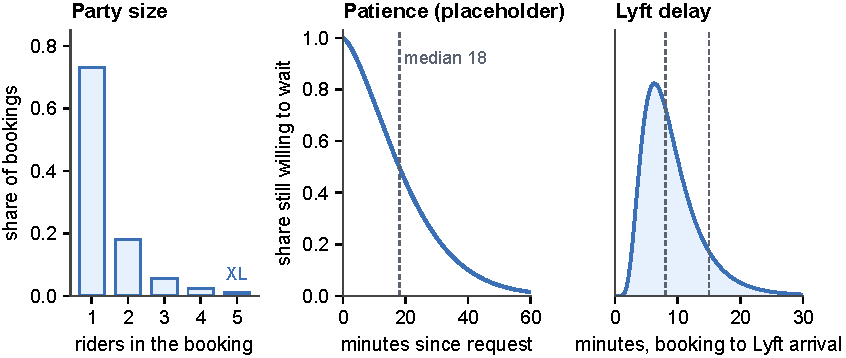
\includegraphics[width=\textwidth]{figures/f4_assumed.pdf}
\caption[Three assumed input distributions]{Three assumed input distributions \Assumed. Left: party-size shares (the base, \D{38}). Middle: the placeholder patience distribution, shown as the share of riders still willing to wait after a given time. Right: the assumed Lyft delay from booking to arrival; dashed lines mark its median (8 min) and P90 (about 15 min). None of these is a measured Hopkins distribution; the curves are drawn from the stated parameters only.}\label{fig:assumed}
\end{figure}

\subsection{No-shows: who is at the curb}\label{sec:noshow}
\begin{blockcard}
\cardrow{Evidence}{2,359 ``No Show'' = 4.7\% of \emph{all} recorded requests \Evidence. JHU: the van waits up to 3 minutes; a Lyft waits no more than 3 minutes.}
\cardrow{Assumption}{Presence is checked only when a vehicle reaches the curb. If the rider is absent, the vehicle waits 180~s and a no-show is recorded; a van no-show frees the van and triggers a re-plan (\D{40}) \Accepted. One hidden presence draw $U_r$ per request and \emph{one} probability $p$ for every mode: the rider is absent if $U_r < p$ (\D{48}(1)). Equality across modes is \Assumed.}
\cardrow{Calculation}{Under the status mapping (Completed = van-completed; ``No Show'' recorded only after a real van arrival; Lyft hand-offs recorded as ``Canceled''): van arrivals $\approx$ 24,095 + 2,359 = 26,454, so $p \approx$ 2,359 / 26,454 $\approx$ 8.9\% per arrival \Derived. The arithmetic is exact; the uncertainty is in the mapping.}
\cardrow{Chosen input}{$p \approx 8.9\%$ \Proposed\ (\D{48}): it depends on a status mapping the team has not accepted.}
\cardrow{Limitation}{No-shows are independent of waiting (a labelled simplification); no late boarding. The frozen inputs' ``4.7\%'' labels and \fn{p_noshow: 0.047} fields are all-request shares; the simulator must not read them (errata, \D{48}(3)).}
\cardrow{Sensitivity}{Separate van / Lyft / XL thresholds (deferred); presence depending on wait, through silent abandonment (\D{42}).}
\end{blockcard}

\textbf{Why the denominator matters.} April's 4.7\% divides by every request, including the roughly 47\% that ended ``Canceled'' before any van came. A probability applied at the curb must divide by the number of curb arrivals instead. \Cref{fig:noshow} shows the two denominators side by side.

\begin{figure}[!htbp]
\centering
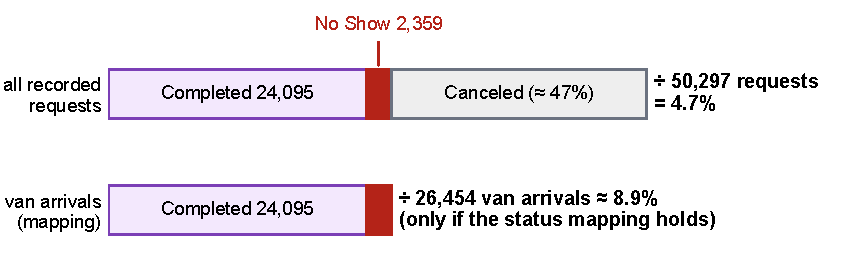
\includegraphics[width=\textwidth]{figures/f3_noshow.pdf}
\caption[Two denominators for the same no-shows]{Two denominators for the same 2,359 no-shows. Top: April's share of all recorded requests \Evidence. Bottom: the rate per van arrival, which holds only if every completed ride and every no-show had exactly one van arrival and ``Completed'' excludes Lyft \Derived. Applying 4.7\% at the curb would use the wrong denominator.}\label{fig:noshow}
\end{figure}

\subsection{Lyft: what happens after a transfer}
\begin{blockcard}
\cardrow{Evidence}{JHU page: the dispatcher sends the Lyft, riders are texted, the Lyft waits no more than 3 minutes. Lyft's driver help: a no-show is recorded only after arrival and the wait timer. No Hopkins data on Lyft delays, failures or XL.}
\cardrow{Assumption}{A lightweight service (\D{43}) \Accepted: transfer decision $\to$ booking after the dispatcher lag $\ell$ $\to$ arrival after a per-request delay $\lambda_r$ $\to$ the same presence test as for vans $\to$ 30~s boarding $\to$ a direct, unpooled ride of $t_0(o,d)\, m_L$. No automatic rebooking after a Lyft no-show or failure. XL uses the same settings as standard Lyft by assumption.}
\cardrow{Chosen input}{$\ell$ = 2 minutes \Assumed; $\lambda_r$ lognormal, median 8 minutes, P90 $\sim$15 minutes \Assumed; failure probability $f = 0$ \Assumed; consent $p_c = 1$, so a decision is a booking request and there is no offer stage (\D{45}).}
\cardrow{Limitation}{Everything numerical about Lyft is assumed. Driver cancellations and re-matching are absorbed into the aggregate delay.}
\cardrow{Sensitivity}{Lyft delay median 5 / 8 / 12 minutes, plus scarcity; lag 0 / 2 / 5 minutes; consent 1.0 / 0.8; dispatcher capacity (at most 3 transfers per 10 minutes); $f > 0$ (\st{lyft_failed}); longer or scarcer XL.}
\end{blockcard}

\textbf{The rules under study.} The Lyft rule is evaluated after every dispatcher solve, at time $\tau$. Only riders still pending with the vans (not committed, not on board) are eligible. Every rule counts waiting from the original request, and the rider's patience keeps running after a transfer (spec §6). \Cref{tab:rules} lists the rules; all are kept and run one at a time (\D{28}) \Accepted.

\begin{table}[!htbp]
\centering\small
\caption[The Lyft transfer rules]{The Lyft transfer rules (\fn{scenario_spec.md} §6). $t_r$ is the request time; ETAs come from the dispatcher's current plan.}\label{tab:rules}
\begin{tabularx}{\textwidth}{@{}P{3.0cm}LP{3.3cm}@{}}
\toprule
\textbf{Rule} & \textbf{Transfers a pending rider when} & \textbf{Information used}\\
\midrule
R0 Never & never (the reference, not the status quo) & none\\
R1($\theta$) Elapsed wait & $\tau - t_r \ge \theta$, with $\theta \in \{10, 15\}$ min & request time\\
R1u(10) Elapsed unassigned & the rider has had no assigned van for $\ge$ 10 min continuously & assignment status\\
R2(15) Predicted total wait & predicted pickup $- t_r >$ 15 min & plan ETAs\\
R3(2) Van vs Lyft & predicted van pickup $> \tau + \ell + 8 + 2$ min & ETAs, typical Lyft delay, lag\\
R4 Congestion-gated (optional) & R2 or R3, only when pending $\div$ available vans $> \kappa$ & board totals\\
\bottomrule
\end{tabularx}
\end{table}

R1 always lets the rider wait $\theta$ minutes first; R2 can transfer at minute one.

\subsection{Patterns, seeds and pairing}
Besides the base recipe, three named patterns stress demand only; fleet, policies and the rules for hidden traits are untouched (\cref{tab:patterns}). Each pattern has its own demand streams, so comparisons \emph{between} patterns are not paired, while rule comparisons \emph{within} a pattern are (\D{49}(6)).

\begin{table}[!htbp]
\centering\small
\caption{Demand patterns (\fn{scenario_spec.md} §3.4).}\label{tab:patterns}
\begin{tabularx}{\textwidth}{@{}P{2.3cm}LL@{}}
\toprule
\textbf{Pattern} & \textbf{What changes} & \textbf{Why it matters for Lyft rules}\\
\midrule
Base & Nothing & Reference\\
Burst & 40\% of the 18:00--19:00 requests inside one 10-minute block & Do rules that act early beat rules that wait?\\
Far-trip & Trips with an end in Peabody/downtown twice as likely (re-normalised) & Long, isolated trips tie up vans and are natural Lyft candidates\\
High load & $\rho \times 1.3$ & Sustained overload: the resource side of transferring\\
\bottomrule
\end{tabularx}
\end{table}

\begin{table}[!htbp]
\centering\small
\caption[Hidden per-request draws]{Hidden per-request draws (\fn{latent.csv}). All are drawn for every request, used or not, from separate seeded streams \Assumed.}\label{tab:latent}
\begin{tabularx}{\textwidth}{@{}P{2.6cm}LP{4.2cm}@{}}
\toprule
\textbf{Draw} & \textbf{Distribution} & \textbf{Used when}\\
\midrule
\fn{patience_s} & Weibull, shape 1.5, median 18 min (placeholder) & the rider is still waiting for a vehicle when it runs out\\
\fn{noshow_u} & Uniform $U_r$; absent if $U_r < p$ & any vehicle reaches the curb\\
\fn{consent_u} & Uniform; accepts Lyft if below $p_c$ (base 1.0) & a transfer is decided\\
\fn{lyft_delay_s} & Lognormal, median 8 min, P90 $\sim$15 min & a transfer is booked\\
\fn{lyft_noshow_u} & generated but unused (\D{41}) & never\\
\fn{eta_noise} & multiplier on the displayed ETA & ETA-dependent patience variant only\\
\bottomrule
\end{tabularx}
\end{table}

% ================================================================== 4
\section{The simulator contract in plain language}\label{sec:contract}

The simulator is the referee. Its rules are written so that two people building it independently would produce the \emph{same} event log from the same inputs. The authoritative text is \fn{scenario_spec.md} §17. The conventions come from the 21 October consolidation review (\D{46}) and are \Proposed: written down and used for the build, but not separately approved by the team. A few further conventions were fixed when the simulator was first built (spec §17.9, \D{52}); they are \Provisional{} and summarised in \cref{sec:conventions}. What has been built and verified is reported in \cref{sec:status}, not here.

\subsection{Time and travel}
\begin{itemize}
\item The clock counts \textbf{integer seconds from 18:00}; every event time is a whole number.
\item There is one base travel table $t_0(i,j)$ in matrix seconds. Van time is $t_0 \times m_v$ and Lyft ride time is $t_0 \times m_L$; each multiplier is applied \emph{exactly once}, then rounded to whole seconds with the same rule as the scenario generator (Python's round-half-to-even), so the hand-check answer keys reproduce exactly (\D{47}(1), a \Correction{} of an earlier double application).
\item \fn{direct_s} in the request file is the unscaled $t_0$ and is used only for reporting. The ride guardrail uses $t_0(o,d) \times m_v$.
\item Base $m_v = m_L = 1.2$ \Assumed; the L1--L4 answer keys use $m = 1.0$, as written in their scenario files.
\end{itemize}

\subsection{Request states and commitment}
A request moves through named states (\cref{fig:lifecycle} in \cref{sec:lifecycle}):
\begin{itemize}
\item \st{pending_van}: known to the dispatcher, not yet committed; it may be reassigned between vans at every re-plan.
\item \st{committed}: a van has \textbf{departed} toward the rider's pickup. Commitment happens at departure, and the van's next stop is then frozen (\D{46}(4)).
\item \st{onboard}, then \st{van_completed} at drop-off; or \st{noshow_van}; or \st{cancel_pending_van} (possible while \st{pending_van} or \st{committed}, that is, until a van reaches the curb).
\item On the transfer path: \st{xfer_hold} (decision made, lag running), then \st{lyft_booked}, then one of \st{lyft_completed}, \st{noshow_lyft}, \st{cancel_after_transfer} or \st{lyft_failed}.
\end{itemize}
An audit invariant must hold at every moment: \textbf{no request is ever in a van route and in a Lyft state at the same time}.

\subsection{What happens when several events share a second}
Integer seconds make ties common. The contract fixes the order by event class (\cref{tab:order}); ties inside a class are broken by request ID, then van ID.

\begin{table}[!htbp]
\centering\small
\caption[Same-second event order]{Same-second event order (\fn{scenario_spec.md} §17.3; \D{46}(2) \Proposed).}\label{tab:order}
\begin{tabularx}{\textwidth}{@{}cP{3.6cm}L@{}}
\toprule
\textbf{Order} & \textbf{Class} & \textbf{Notes (spec §17.3)}\\
\midrule
10 & Drop-offs (van and Lyft) & Frees seats before anything else is decided\\
20 & Curb arrivals (van and Lyft) & Ends the patience clock, so an arrival wins a same-second tie with the deadline; the presence test is made here\\
30 & Service ends & Boarding dwell ends; a no-show is recorded after the 180-s curb wait\\
40 & Van on duty / off duty & --\\
50 & New requests & --\\
60 & Patience checks & A rider still \st{pending_van}, \st{committed} (van driving to the curb, not yet arrived), \st{xfer_hold} or \st{lyft_booked} whose deadline has passed cancels\\
70 & Lyft bookings & \st{xfer_hold} becomes \st{lyft_booked} at decision + $\ell$\\
80 & Epoch & Van solve $\to$ evaluate the Lyft rule once $\to$ apply transfers $\to$ re-solve once if any transfer\\
90 & Departures & Vans leave toward their next stop; this is the moment of commitment\\
\bottomrule
\end{tabularx}
\end{table}

\subsection{Epochs: when the dispatcher re-plans}
\begin{itemize}
\item There is \textbf{one epoch per distinct second} that has a trigger. Triggers are a new request, a cancellation or no-show \emph{of a request in van planning}, a transfer (handled inside the epoch by the re-solve), a van going on or off duty, and a periodic tick every 120~s anchored at $t = 0$ (\D{46}(3); spec §17.4). Lyft-side events (booking, Lyft arrival, Lyft no-show, Lyft drop-off) never trigger an epoch, because they cannot change a van plan (\D{52}).
\item \textbf{Zero simulated latency:} a plan computed at time $\tau$ takes effect at $\tau$. The solver is limited by deterministic node or iteration budgets; wall-clock time is logged as a diagnostic and never changes a plan, so runs are reproducible on any machine (\D{46}(5)).
\item A request that no route in the current plan serves stays \textbf{pending}. It still carries a \textbf{tentative ETA}, its cheapest feasible insertion computed outside the solver, and the log records why it is pending (competition with other requests, or the candidate cap). Lyft rules that read ETAs read this value (\D{47}(3)).
\end{itemize}

\subsection{Transfers and the Lyft service}
\begin{itemize}
\item \textbf{Consent.} In the base, $p_c = 1$, so every decision is a booking request. Where $p_c < 1$ (L4 uses 0.9; the consent sensitivity 0.8), a decision is an \emph{offer}: a rider whose \fn{consent_u} exceeds $p_c$ declines, stays with the vans, is never offered again, and the decline is counted.
\item \textbf{Transfer at the decision.} A consented decision at $\tau$ removes the request from van planning \emph{at $\tau$}, atomically, and puts it in \st{xfer_hold}. Leaving at the booking instead was rejected, because with $\ell$ = 120~s equal to the tick a van could be sent to a rider who is about to leave by Lyft.
\item \textbf{Booking after the lag.} At $\tau + \ell$ the booking is placed. If the rider's deadline falls inside the lag, the outcome is \st{cancel_after_transfer} and \textbf{no booking} is counted.
\item \textbf{Arrival and ride.} The Lyft arrives at booking + $\lambda_r$. The presence test uses the same $U_r$ and $p$ as for vans. A present rider boards (30~s dwell, as for vans) and rides directly; an absent one becomes \st{noshow_lyft} after 180~s.
\item Parties of one to four book a standard Lyft; parties of five book an XL. Every count is kept separately for the two. There is no automatic rebooking.
\item \textbf{The pickup instant, in both modes,} is the curb arrival of the vehicle the rider boards; the 30-s boarding dwell follows. So the wait is $W$ = curb arrival $-$ request time, and the ride $H$ = drop-off arrival $-$ curb arrival, which includes the dwell. This is the convention of the L1--L4 answer keys (spec §17.5). For riders who do not board, the curb arrival is still recorded, and no wait-to-pickup is reported for them.
\end{itemize}

\begin{figure}[!htbp]
\centering
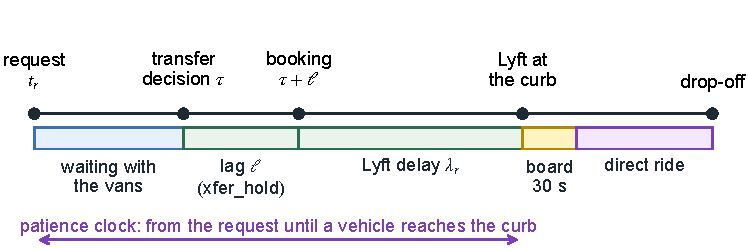
\includegraphics[width=\textwidth]{figures/f8_transfer.pdf}
\caption[Timeline of a transferred rider]{Timeline of a transferred rider (not to scale). The request leaves van planning at the decision; the booking is placed one lag later; the Lyft arrives after the rider's hidden delay $\lambda_r$. The rider's patience clock keeps running from the original request until a vehicle reaches the curb. The wait is measured from the original request to that curb arrival, the pickup instant; a transfer never resets the clock.}\label{fig:transfer}
\end{figure}

\subsection{Shifts and closing}
After the arrival window, vans stay on duty until every accepted request is resolved (\D{36}; \D{46}(6)). For the L5 rehearsal level, the frozen \fn{avail_end_s} = 3600 is read as the end of the arrival window, not a shift end. For tapering cases (L7), the shift-end grace is $g = 0$. Every run must end with \st{unresolved_close} = 0.

\textbf{The shift-end rule itself is open} \Open. The documents give two wordings: a new pickup must \emph{start} before the van's end (spec §17.6), or its \emph{drop-off} must end before it (\fn{model_design.md} §3.3). It matters only for tapering cases (L7), is not implemented, and is to be settled before L7 is built. Riders already on board are always finished.

\subsection{Inputs the simulator must not read}
\begin{itemize}
\item \fn{p_noshow} in \fn{scenario.json} and the ``DERIVED rate 4.7\%'' label (errata, \D{48}(3)); $p$ comes from the behaviour configuration.
\item \fn{lyft_noshow_u} (unused under the shared presence draw, \D{41}).
\item \fn{eta_noise}, except in the ETA-dependent patience variant.
\end{itemize}
More generally, no policy may see future requests or any hidden draw. The only exception is the clearly labelled hindsight benchmark H on tiny instances (\fn{model_design.md} §3.1).

\subsection{Required logs}
\begin{itemize}
\item \textbf{Event log:} every event with time, class, request, van, old state and new state.
\item \textbf{Epoch log:} the trigger, open requests, candidates per van, solver status and gap, the chosen plan, pending requests with their reason and tentative ETA, and each Lyft decision with the quantity the rule read.
\item \textbf{Plan audit} after every epoch: capacity, precedence, commitments, shift ends, the guardrail (no new or increased violation) and the transfer invariant.
\item \textbf{Run manifest:} input hashes, policy file, code version, solver version and settings.
\end{itemize}

\subsection{Conventions fixed when the simulator was built}\label{sec:conventions}
Building the simulator required a few rules the contract had not spelled out. They are recorded in spec §17.9 and \D{52}, and are \Provisional{} (team review pending):
\begin{itemize}
\item \textbf{Moving vans} can be re-routed only at a stop; once a van departs toward a stop it completes that leg.
\item \textbf{Cancelled pickup:} if the rider cancels while the van is driving, the van still reaches the curb, finds no rider and is free at once (no dwell).
\item \textbf{No-show:} recorded 180~s after curb arrival; the van then leaves without dwell. During that wait the dispatcher sees the van free at arrival + 180~s without the rider, which is what the driver observes (no late boarding is assumed).
\item \textbf{Planning a committed pickup:} the dispatcher plans as if the rider boards, because it cannot see the presence draw.
\item \textbf{0-s legs} (consecutive stops at the same point): the arrival is processed in the same second, after that second's departures. This is the one exception to the class order of \cref{tab:order}.
\item \textbf{Ties inside a class} are broken by key, so request IDs (R\ldots) sort before van IDs (V\ldots).
\item \textbf{M0 Lyft harness:} in L4 the transfer rules act only before 18:15 (900~s), the hand-checkable window. Lyft rules running alongside the dispatcher after 18:15 are milestone M2.
\end{itemize}

\subsection{Terminal states and the dashboard view}
Each request ends in exactly one terminal state \Simulated: \st{van_completed}, \st{lyft_completed}, \st{cancel_pending_van}, \st{cancel_after_transfer}, \st{noshow_van}, \st{noshow_lyft}, \st{lyft_failed} (sensitivity only) or \st{unresolved_close} (must be zero). A transfer is an event, not a completion. Wait is always the pickup instant (curb arrival of the boarding vehicle, either mode) minus request time. For calibration only, a dashboard-comparable view is derived: ``Completed'' = van-completed; ``Canceled'' = rider cancellations + transfers (spec §5).

\subsection{Designed checks: the level ladder}
Before any experiment, the simulator must reproduce hand-computed answers on small, designed cases \Designed. The answer keys were computed by the scenario generator from the travel matrix and recomputed in tests. The M0 simulator now reproduces the L1--L3 keys to the second and the L4 pre-18:15 Lyft key (\cref{sec:status}). \Cref{tab:ladder} summarises the ladder.

The L4 key covers R0 plus five active rule cases: R1(10), R1(15), R1u(10), R2(15) and R3(2). Across those five rule runs there are 22 transfer decisions (R1(10) 3, R1u(10) 3, R2(15) 8, R3(2) 8; 4 of them by XL) and 4 consent declines (one per rule, except R1(15), which makes no decision before 18:15). These are totals across separate rule runs, not counts for one night.

\begin{table}[!htbp]
\centering\small
\caption[The level ladder]{The level ladder (\fn{scenario_spec.md} §8). L1--L4 check correctness \Designed; L5 rehearses the pipeline; only L6--L7 answer the research question \Simulated.}\label{tab:ladder}
\begin{tabularx}{\textwidth}{@{}P{1.0cm}P{4.3cm}L@{}}
\toprule
\textbf{Level} & \textbf{Size} & \textbf{What it checks}\\
\midrule
L1 & 2 vans, 16 requests, one open at a time & Every pickup and drop-off time, to the second\\
L2 & L1 + 2 designated no-shows & The 180-s curb wait, no-show handling, re-plan\\
L3 & L1 + designated patience values & The cancel-while-waiting path\\
L4 & 2 vans, 16 requests in $\sim$20 min; vans on duty at 18:15; one party of five & Lyft bookkeeping before 18:15: 22 transfers (4 by XL) and 4 declines, summed over five rule runs\\
L5 & 2 vans, 28 requests in 60 min, $\ge$ 40\% in a burst; 30 seeds & Dress rehearsal: pairing, metrics, explanations; too small for conclusions\\
L6 & 5 vans constant, 168 requests + backlog; sixth van on the same requests & Main Lyft-rule experiments (6 rules $\times$ 4 patterns $\times$ 2 fleet levels $\times$ 30 nights)\\
L7 & 5--6 vans, 18:00--02:00 + backlog (counts not yet derived) & Confirmatory runs with taper and shift ends\\
\bottomrule
\end{tabularx}
\end{table}

Stated in advance: L1--L4 should show almost no algorithm differences, because the load is low. Conclusions come only from L6--L7.

% ================================================================== 5
\section{The dispatcher's mathematics}\label{sec:math}
This section explains how the van dispatcher scores and chooses its plans: first in words, then in symbols, then through a small worked example. It ends with what the word ``optimal'' can and cannot mean here.

\subsection{The idea in words}
At each epoch the van dispatcher looks at every van and every rider not yet picked up. It decides who each van picks up next and in what order. Only each van's next move is carried out; the rest is a plan that the next epoch may change. This is \emph{rolling-horizon re-optimization} of a dynamic dial-a-ride problem, a standard framing in the literature (Berbeglia, Cordeau and Laporte 2010; Ho et al.\ 2018) and consistent with TransLoc's 2016 description of its engine, which re-planned on events and every two minutes.

The dispatcher plans only from what a real dispatcher could see: requests already revealed, van states, travel tables and published rules. It never sees future requests or riders' hidden traits.

\subsection{What a ``good'' plan means}
A plan is scored in \textbf{points}, which are penalised passenger-minutes; lower is better. The points are \emph{priorities, not money}. Four ideas make up the score.

\textbf{Waiting counts more the longer someone has waited.} Each passenger's total wait $W$ (from the original request, so time already spent waiting counts) is charged a convex penalty $\varphi(W)$: the first five minutes cost 1 point per minute, the next five 2.5, then 5, 10 and finally 20 points per minute beyond 20 minutes (\cref{fig:phi}). Thus $\varphi(5) = 5$, $\varphi(10) = 17.5$, $\varphi(15) = 42.5$ and $\varphi(20) = 92.5$. The break-points at 15 and 20 minutes follow the published Homewood targets. Only the 3--10 minute region is constrained by evidence: TransLoc's 2016 example prefers cutting one minute from a 10-minute wait over two minutes from a 5-minute wait, so $\varphi(10) - \varphi(9) > \varphi(5) - \varphi(3)$. A straight line fails that test (1 is not more than 2); the chosen slopes pass it (2.5 > 2). The rest of the shape is our choice \Assumed.

\begin{figure}[!htbp]
\centering
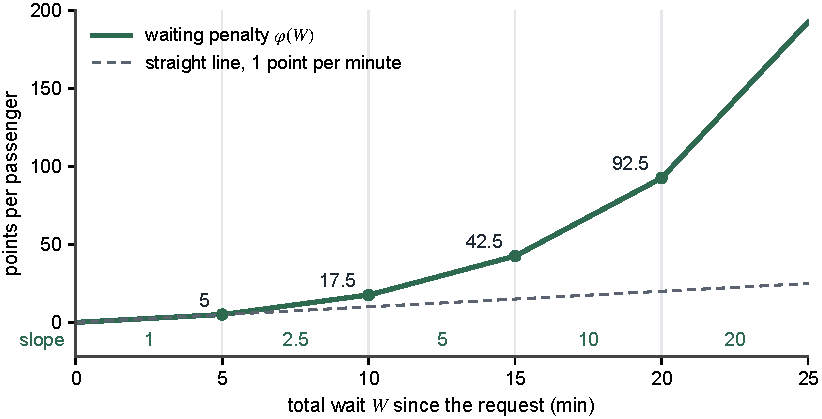
\includegraphics[width=\textwidth]{figures/f5_phi.pdf}
\caption[The convex waiting penalty]{The convex waiting penalty $\varphi(W)$ per passenger (\D{29} \Accepted). The slope rises at 5, 10, 15 and 20 minutes, so a minute of waiting costs more the longer the rider has already waited. The dashed line shows a constant 1 point per minute for comparison.}\label{fig:phi}
\end{figure}

\textbf{Riding counts, but less than waiting.} Each passenger-minute on board costs $\beta = 0.5$ points. Because $\beta = 0.5$ and every slope of $\varphi$ is at least 1, a waiting minute always outweighs a riding minute, from minute zero (\D{47}(5), a \Correction{} of earlier wording). This expresses ``waiting matters more'' as a marginal priority, not an absolute one \Assumed.

\textbf{Driving costs a little.} Each route-kilometre costs $\gamma = 0.1$ points, a small tie-breaker against pointless driving \Assumed.

\textbf{Nobody rides unreasonably long.} The ride guardrail for request $r$ is
\begin{equation}
G_r = \max\bigl(25\ \text{min},\ 2\,T_r + 5\ \text{min}\bigr),
\end{equation}
where $T_r$ is the direct van time \Assumed. The form is \Accepted{} (\D{29}). The enforcement convention is \Proposed{} (\D{47}(2)): no candidate route may \emph{create or increase} a guardrail violation; the ``committed work only'' route is exempt, and any violation already locked into committed work is charged a very large penalty $\Psi$ per passenger-minute over the guardrail and logged. The 20-minute published target is a reporting threshold, not the guardrail, because a hard 20 would be stricter than the service delivers (April's ride P90 is about 24 minutes).

\textbf{Leaving a request pending has a price.} A request left unassigned for this epoch costs
\begin{equation}
\pi_r = q_r\, \varphi\bigl(W_r^{\text{next}}\bigr) + M ,
\end{equation}
where $W_r^{\text{next}}$ is its wait if picked up no earlier than the next epoch and $M$ is large. With a large $M$ the solver first serves as many requests as it can within its candidate routes, then minimises points. A request can still be left pending when routes compete for it (taking it would mean dropping two others) or when the candidate cap leaves it out (\D{47}(3), a \Correction{} of an earlier claim that this could not happen). $M$ must be the same for every dispatcher, otherwise a dispatcher could look good by starving hard requests. In the implementation $M$ is set at each epoch to an explicit bound that guarantees every optimal plan leaves the fewest requests pending that the candidate set allows (\D{52}).

\textbf{An open question about this price} \Open. The price charges a pending request as if it were picked up at the next epoch, earlier than any physically possible pickup, while a served request is charged its real, later pickup. When the candidate cap binds, the cheapest requests to defer can therefore be those that would be picked up late, often the longest waiters, which works against the purpose of the convex $\varphi$ (\D{53}). Two alternatives keep the $M$ bound valid: price a pending request at the earliest time any van could physically reach it (A), or at the wait it would have if appended to the end of a van's chosen route (B). Neither is implemented; a team decision is needed before the Lyft-rule experiments. \Cref{sec:status} shows where M1 met this property.

\subsection{The route-selection model}
\textbf{Candidate routes.} For each van $v$, routes $k$ are built in advance. Each is an ordered stop list that starts at the van's committed next stop, keeps all drop-offs of riders already on board and any committed pickup, and adds a subset $S_k$ of open requests (pickup before drop-off). The ``committed work only'' route is always included, so a feasible plan always exists. Capacity, pickup-before-drop-off, commitments, shift ends and the guardrail are all enforced while routes are built; each candidate is simulated forward to give every rider's pickup and drop-off times.

\textbf{Route cost.} With $q_r$ passengers, wait $W_r$ and ride time $H_r$:
\begin{equation}
c_{vk} = \sum_{r \in S_k \cup C_v} q_r\, \varphi(W_r) \;+\; \beta \sum_{r\ \text{on route}} q_r H_r \;+\; \gamma\, \text{km}_k \;+\; \Psi \sum_{r} q_r \bigl(H_r - G_r\bigr)^{+} .
\end{equation}
$C_v$ is the van's committed pickup. Because $\varphi$ is evaluated while route costs are computed, outside the solver, the optimization stays linear whatever shape $\varphi$ has.

\textbf{The choice.} With $y_{vk} = 1$ if van $v$ uses route $k$, and $u_r = 1$ if open request $r$ stays pending:
\begin{equation}
\begin{aligned}
\min\ & \sum_{v}\sum_{k} c_{vk}\, y_{vk} + \sum_{r} \pi_r\, u_r\\
\text{s.t. } & \textstyle\sum_{k} y_{vk} = 1 && \text{for every van } v \quad\text{(one route per van)}\\
& \textstyle\sum_{v,\,k:\ r \in S_k} y_{vk} + u_r = 1 && \text{for every open request } r \quad\text{(one van, or pending)}\\
& y_{vk},\ u_r \in \{0, 1\}.
\end{aligned}
\end{equation}
This is the pattern of Alonso-Mora et al.\ (2017), with ``drop the request'' replaced by ``defer it at price $\pi_r$''.

\textbf{The candidate set.} For tractability, each candidate route may add only a few open requests, and every open request gets at least one single-insertion candidate on every van that can feasibly take it (\D{47}(3)). The settings used for milestones M0--M1 are recorded in \D{52}: every subset of at most $K = 3$ open requests (new pickups) per van, each subset getting its best stop order found exactly. Under the \D{52} amendment that best order covers all of the van's stops, including the drop-offs of riders already on board. \D{52} also replaces the earlier wording that counted the cap relative to the van's previous plan. These settings are implemented and \Provisional{} (team review pending); they change the candidate set, not the objective.

\subsection{Worked example: why the long waiter goes first}
One empty van, two open requests, both routes 10~km, dwell omitted for clarity. Request r1 has one passenger who has already waited 8 minutes; r2 has two passengers who have waited 1 minute. The example is taken from methodology §6.

\begin{figure}[!htbp]
\centering
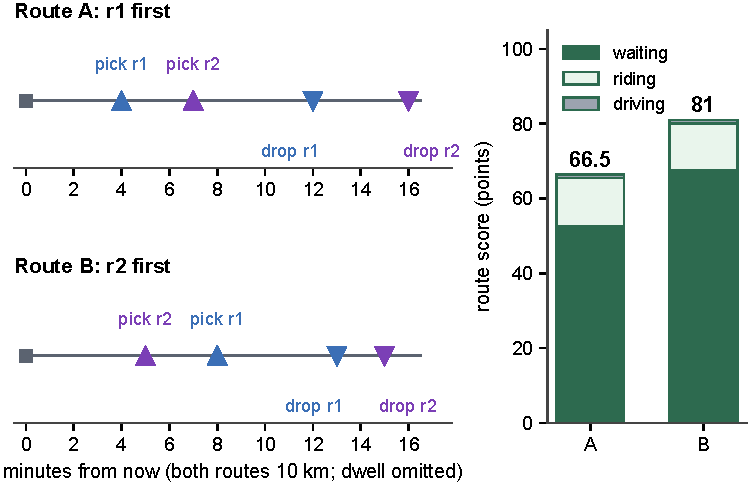
\includegraphics[width=\textwidth]{figures/f6_example.pdf}
\caption[Worked example: two candidate routes]{Worked example: two candidate routes for one van. Triangles pointing up are pickups, down are drop-offs. Right: each route's score split into waiting, riding and driving points. The arithmetic is in \cref{tab:example}.}\label{fig:example}
\end{figure}

\begin{table}[!htbp]
\centering\small
\caption[Worked example arithmetic]{Worked example arithmetic. Times in minutes; $\varphi(12) = 5 + 12.5 + 10 = 27.5$, $\varphi(8) = 5 + 7.5 = 12.5$, $\varphi(16) = 42.5 + 10 = 52.5$, $\varphi(6) = 5 + 2.5 = 7.5$. All values checked for this document.}\label{tab:example}
\begin{tabularx}{\textwidth}{@{}P{2.4cm}LL@{}}
\toprule
 & \textbf{Route A: r1 first} & \textbf{Route B: r2 first}\\
\midrule
Stops & r1 at 4, r2 at 7, drop r1 at 12, drop r2 at 16 & r2 at 5, r1 at 8, drop r1 at 13, drop r2 at 15\\
Waits & $W_1 = 8 + 4 = 12$; $W_2 = 1 + 7 = 8$ & $W_1 = 8 + 8 = 16$; $W_2 = 1 + 5 = 6$\\
Rides & $H_1 = 12 - 4 = 8$; $H_2 = 16 - 7 = 9$ & $H_1 = 13 - 8 = 5$; $H_2 = 15 - 5 = 10$\\
Waiting & $1 \cdot 27.5 + 2 \cdot 12.5 = 52.5$ & $1 \cdot 52.5 + 2 \cdot 7.5 = 67.5$\\
Riding & $0.5\,(1 \cdot 8 + 2 \cdot 9) = 13.0$ & $0.5\,(1 \cdot 5 + 2 \cdot 10) = 12.5$\\
Driving & $0.1 \cdot 10 = 1.0$ & $0.1 \cdot 10 = 1.0$\\
\midrule
\textbf{Total} & \textbf{66.5} & \textbf{81.0}\\
\bottomrule
\end{tabularx}
\end{table}

The dispatcher picks A. The rider who has already waited 8 minutes goes first, even though r2 carries two passengers and B gives slightly less riding. Passenger weighting gives a group's combined delay more weight, but it does not automatically put groups first: the plan with the lowest total wins. The convex $\varphi$ is what protects the long waiter: in B, r1's wait crosses 15 minutes, where each minute costs 10 points. Both rides are far below the 25-minute guardrail. This is a \Designed{} illustration computed by hand, not a simulation output.

\subsection{What ``optimal'' means here}
\begin{callout}
The restricted route-selection model C is \textbf{optimal over its candidate set, subject to solver status}. It is not ``optimal over all routes'', and not ``optimal for the evening''.
\end{callout}
Three reasons keep the claim narrow:
\begin{itemize}
\item \textbf{Candidate set.} C chooses only among the routes that were built. A route outside the set is never considered.
\item \textbf{Solver status.} Optimality holds only when the solver closes its gap. The proposed settings are a relative gap of 0, a small absolute gap and a node limit, with $M$ and $\Psi$ set and recorded before any comparison (\D{47}(4) \Proposed). The values used in M0--M1 (\D{52} and amendments 2--3, \Provisional) are: HiGHS with one thread and a fixed seed, relative gap 0, absolute gap below one cost unit, a node limit of 100,000 as the only budget, and $\Psi$ = 1000 points per passenger-minute. A wall-clock safety limit stops the run with an error rather than letting wall time change a plan. If the node budget is reached, the best plan found is executed and labelled \emph{feasible, unproven}, and no pending reasons are established for that epoch. A solve that ends with no plan at all (\emph{failed}) executes committed work only and is logged. A solver error or an infeasible model stops the run (infeasibility cannot occur, because the committed-only routes are always feasible); T is never invoked. None of these cases occurred in the M0--M1 runs. An epoch with nothing to decide is labelled \emph{empty}. Status and gap are logged at every epoch, and a plan audit after every epoch stops the run on any violation (\D{52} amendment 3).
\item \textbf{One epoch at a time.} Each epoch is solved with what is known then. Per-epoch optimality is not whole-evening optimality.
\end{itemize}
A difference between C and the heuristic T measures the search alone only when both search the same candidate set with the same objective (\D{47}(5)).

\subsection{The dispatchers and the held-fixed choice}
\begin{table}[!htbp]
\centering\small
\caption[Van dispatchers]{Van dispatchers (\fn{model_design.md} §6.1, with the \D{51} update).}\label{tab:players}
\begin{tabularx}{\textwidth}{@{}P{2.6cm}LP{3.6cm}@{}}
\toprule
\textbf{Dispatcher} & \textbf{Definition} & \textbf{Role}\\
\midrule
C, route selection & The model above, solved with HiGHS each epoch over a recorded candidate set & Provisionally the held-fixed dispatcher (\D{51}); built and verified on L1--L4\\
T, TransLoc-like & Same model, solved by insertion and local search with a fixed iteration budget & Later robustness variant or development contingency; not built\\
T$-$ & T without reassignment and/or a 300-s cadence & Baseline-uncertainty variant\\
G, greedy & Insert each new request at its cheapest position on arrival; never reassign & Floor; robustness check\\
H, hindsight & Node-arc model with full knowledge of a tiny night & Information bound on L1 only\\
\bottomrule
\end{tabularx}
\end{table}

\textbf{Status (\D{51}).} C is \Provisional{}: the team \emph{intends} to hold it fixed in the main Lyft-rule experiments, conditional on a later benchmark showing it fits the time budget on the full workload. It does not claim to reproduce Hopkins' proprietary dispatcher; it shares the published structure (event plus periodic re-planning, reassignment, convex waiting penalty). \textbf{T is a development contingency, never an automatic runtime fallback.} If C proves unsuitable, the team decides whether to change the fixed dispatcher before experiments are frozen.

\textbf{The Lyft rule is a separate module.} It runs after each dispatcher solve and reads the board: each open request's request time, party size, assignment state and predicted van pickup. Keeping it separate mirrors Hopkins' human dispatcher, keeps policy apart from algorithm, stays interpretable and needs no price for a Lyft trip. An integrated variant (Lyft as a third option inside the solve, as in Grahn et al.\ 2023) is deferred.

\textbf{Weighted rather than lexicographic.} A strict ``waiting first, always'' ordering risks unbounded on-board detours; the weighted form trades them at an explicit, swept rate ($\beta$ = 0.25 / 0.5 / 1). The lexicographic form is kept as a variant to show the frontier (\fn{model_design.md} §4.2).

% ================================================================== 6
\section{One request's lifecycle}\label{sec:lifecycle}

This section follows a single request through the system. It describes the rules, not a simulated night: no times or outcomes below are \Simulated.

\begin{figure}[!htbp]
\centering
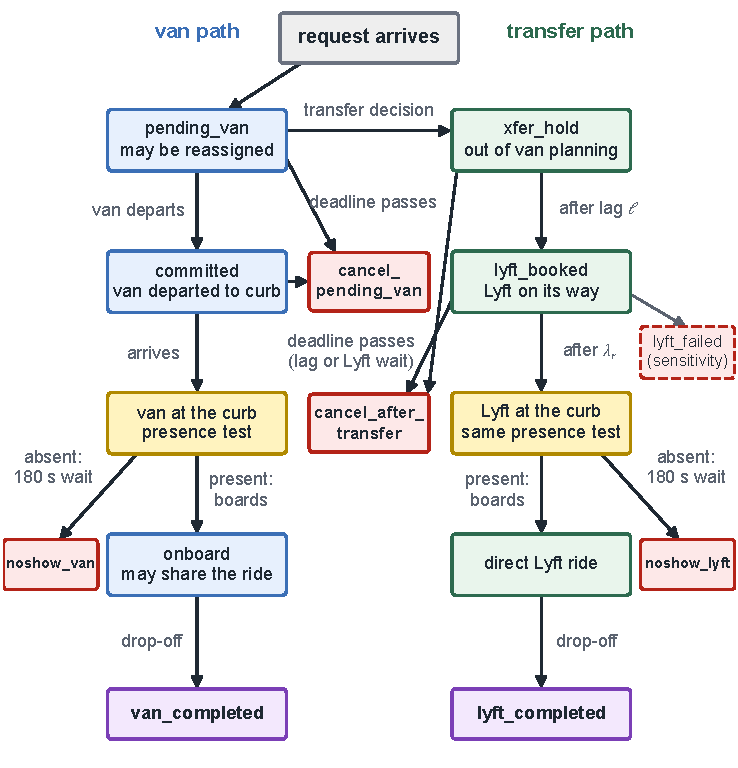
\includegraphics[width=\textwidth]{figures/f7_lifecycle.pdf}
\caption[The life of one request]{The life of one request. Left: the van path. Right: the transfer path. Red boxes are terminal outcomes; the dashed box is used only in a sensitivity case. ``Deadline passes'' is the hidden patience deadline. Arrows follow the states and patience checks of \fn{scenario_spec.md} §17.2--17.3; a rider can cancel both while still \st{pending_van} and while \st{committed} (van driving to the curb).}\label{fig:lifecycle}
\end{figure}

\subsection{The van path}
\begin{enumerate}
\item \textbf{Request.} The request is revealed at its request time and joins the next epoch as \st{pending_van}. Its hidden traits (patience, presence, consent, Lyft delay) are already fixed in the scenario file but stay invisible to the dispatcher and the Lyft rule.
\item \textbf{Planning.} At every epoch the dispatcher may place it on a van's route, move it to another van, or leave it pending with a tentative ETA. The Lyft rule then reads its waiting time and ETA.
\item \textbf{Commitment.} When a van departs toward its pickup, the request becomes \st{committed}: the van's next stop is frozen and it can no longer be reassigned or transferred.
\item \textbf{Curb arrival and presence test.} When the van reaches the curb, the patience clock stops; this curb arrival is the pickup instant that ends the wait. The simulator compares the rider's presence draw $U_r$ with $p$. Present: the rider boards (30~s dwell) and becomes \st{onboard}. Absent: the van waits 180~s, the outcome is \st{noshow_van}, the van leaves without dwell and the dispatcher re-plans.
\item \textbf{Cancellation.} If the rider's deadline passes while still \st{pending_van}, or while \st{committed} with the van on its way, the outcome is \st{cancel_pending_van}. A van already driving still reaches the empty curb and is then free at once (spec §17.9).
\item \textbf{Drop-off.} The van may pick up others on the way, within capacity and the guardrail. At drop-off the outcome is \st{van_completed}; the wait is curb arrival minus request time, and the ride is drop-off minus curb arrival (it includes the boarding dwell).
\end{enumerate}

\subsection{The transfer path}
\begin{enumerate}
\item \textbf{Decision.} After a dispatcher solve, the Lyft rule may decide to transfer the pending request. In the base every decision is accepted; with $p_c < 1$ the rider may decline and stay with the vans.
\item \textbf{Hold.} The request leaves van planning at once (\st{xfer_hold}). If the deadline passes during the lag: \st{cancel_after_transfer}, and no booking is counted.
\item \textbf{Booking.} One lag later the Lyft is booked (\st{lyft_booked}), standard or XL by party size.
\item \textbf{Arrival.} The Lyft reaches the curb after the hidden delay $\lambda_r$; the patience clock stops; the same presence test applies. Absent: \st{noshow_lyft} after 180~s. If the deadline passes before arrival: \st{cancel_after_transfer}.
\item \textbf{Ride.} The rider boards and rides directly; the outcome is \st{lyft_completed}. The wait still counts from the original request.
\end{enumerate}

\subsection{Where each hidden trait enters}
\begin{table}[!htbp]
\centering\small
\caption{Where each hidden trait turns into an outcome.}\label{tab:traits}
\begin{tabularx}{\textwidth}{@{}P{3.2cm}LP{4.2cm}@{}}
\toprule
\textbf{Hidden trait} & \textbf{Applied at} & \textbf{Possible outcome}\\
\midrule
Patience deadline & Patience checks (order 60) while waiting & \st{cancel_pending_van} or \st{cancel_after_transfer}\\
Presence draw $U_r$ & The first curb arrival of any vehicle & boarding, or a no-show after 180~s\\
Consent draw & A transfer decision, only when $p_c < 1$ & stays with vans; decline counted\\
Lyft delay $\lambda_r$ & Booking & Lyft curb arrival time\\
\bottomrule
\end{tabularx}
\end{table}

Because these traits are drawn once per request and shared by every rule, a rider who would have been absent at the curb is absent whichever vehicle comes. Only the waits that a rule produces can change whether that rider is still there to be tested.

% ================================================================== 7
\section{Implementation status, provisional assumptions and next milestones}\label{sec:status}
This section reports what the first simulator milestone (M0--M1, 22 October 2026) built and verified, taken from \fn{scenario_methodology.md} v1.1 §7--§9. It keeps two things apart: what has been \textbf{verified} and what is only \textbf{planned}.

\begin{callout}[What this section does and does not show]
Only designed validation cases (L1--L4, plus a run-time probe on one L5 night) have been simulated. The outcomes below are \Simulated{} outcomes of a \Designed{} case, not evidence about the real service. \textbf{No Lyft-rule comparison has been run, and no rule has won.}
\end{callout}

\subsection{What was built}
The code lives in \fn{src/sim/}, with settings recorded in \D{52} and its amendments:
\begin{itemize}
\item \textbf{Input loader:} reads the frozen scenario files read-only and refuses to run if a content hash differs from the frozen record.
\item \textbf{Event engine (the referee):} owns the clock, the same-second order of \cref{tab:order}, every request state and the hidden rider traits, which it applies only when their event happens.
\item \textbf{Dispatcher C:} for each van, every subset of at most three open requests with its best order of all stops (found exactly), then the selection model of \cref{sec:math} solved by HiGHS, with the explicit $M$ bound, exact integer costs, status handling and a fixed tie rule.
\item \textbf{Lyft rules:} exercised only before 18:15 in L4 (the M0 scope).
\item \textbf{Runner:} writes the event log, the epoch log, per-request outcomes, a run manifest and a readable narrative.
\end{itemize}

\subsection{What was verified}
\begin{table}[H]
\centering\small
\caption[What M0--M1 verified]{What M0--M1 verified (\fn{scenario_methodology.md} v1.1 §7).}\label{tab:verified}
\begin{tabularx}{\textwidth}{@{}P{3.2cm}L@{}}
\toprule
\textbf{Check} & \textbf{Result}\\
\midrule
L1--L3 answer keys & Every request's van, curb arrival, pickup, wait, drop-off, ride, no-show time and cancellation time reproduced \textbf{to the second}, compared with the hand-check sheets by two independent test files\\
L4 Lyft mechanics before 18:15 & For each of the five active rule cases, the transfer and decline sets, decision, booking (+120~s), Lyft pickup (+480~s), wait, drop-off and XL class match: 22 transfers (4 XL) and 4 declines in total across the five rule runs\\
Route selection & All 46 L4 R0 epochs and all L1--L3 epochs solved to proven optimality over the candidate set. Under the current candidate default, the MILP's choice equals full enumeration of compatible candidate combinations on all 46 L4 R0 epochs (151,710 combinations), including the tied epoch and the fewest pending requests. An earlier independent math review found the same on its own runs, made under the earlier fixed drop order\\
Best order per subset & For 40 van states of the L4 R0 run, every subset of at most two requests and a sample of 80 subsets of three (1,130 subsets, 113,879 stop orders): each candidate's cost equals the brute-force minimum over all feasible orders. Not every subset of three was brute-forced\\
Invariants & One terminal state per request; no request both in a van route and a Lyft state; capacity; committed pickups served by the committing van; no ride over the guardrail in these runs\\
Hidden traits & The dispatcher's observation has no hidden-trait fields; changing patience values that never fire leaves plans unchanged\\
Reproducibility & Two runs give identical event logs and epoch records (wall times excluded); frozen inputs unchanged\\
Test suite & 105 tests pass on 22 October: 46 pre-existing scenario tests, 32 engine tests and 27 independent verification tests\\
Integrated review & Ready to hand to the team once its should-fix items were addressed; all were addressed on 22 October (status labels, plan audit, wording)\\
\bottomrule
\end{tabularx}
\end{table}

\subsection{What M1 showed on L4 under R0}
L4 is a designed case: two vans come on duty at 18:15, when nine requests are already waiting. Under R0 (no transfers), the run showed the following \Simulated:
\begin{itemize}
\item At 18:15 the MILP jointly assigns three requests to each van (the cap $K = 3$), sequences them, and leaves three pending, with the cap recorded as the reason (\cref{tab:plan1815}).
\item The plan changes at most epochs while the queue lasts, because uncommitted requests are reassigned; committed pickups never move.
\item All 16 riders are delivered by 19:10. Waits range from 1.2 to 44.4 minutes; the longest ride is 24.9 minutes, within the 25-minute guardrail.
\item Run time was about 27~s for the evening (slowest epoch about 8~s). On one L5 night (28 requests with a burst) all 86 epochs were solved to optimality. Wall times are diagnostics only; simulated solver latency is zero.
\end{itemize}

\begin{table}[H]
\centering\small
\caption[The 18:15 plan in L4 under R0]{The plan chosen at 18:15 in L4 under R0 \Designed\ \Simulated. Times are the curb arrivals planned at 18:15; later epochs revised some of them. Points use $\varphi$ and the party size. The three pending requests are priced at the next tick (18:16:00), excluding $M$. Re-derived for this document from \fn{outputs/sim/L4_R0/epochs.jsonl}; they match the run's narrative. A mirror plan (the vans swapped) scores the same.}\label{tab:plan1815}
\begin{tabularx}{\textwidth}{@{}llrrrrL@{}}
\toprule
\textbf{Van} & \textbf{Request} & \textbf{Party} & \textbf{Requested} & \textbf{Planned curb} & \textbf{Wait} & \textbf{Points}\\
\midrule
V1 & R001 & 3 & 18:00:00 & 18:17:44 & 17:44 & 209.50\\
V1 & R003 & 1 & 18:00:20 & 18:21:33 & 21:13 & 116.83\\
V1 & R008 & 1 & 18:09:40 & 18:25:17 & 15:37 & 48.67\\
V2 & R004 & 2 & 18:01:40 & 18:18:48 & 17:08 & 127.67\\
V2 & R007 & 1 & 18:09:40 & 18:21:48 & 12:08 & 28.17\\
V2 & R009 & 1 & 18:13:50 & 18:23:08 & 9:18 & 15.75\\
\midrule
pending & R002 & 5 & 18:00:00 & (next tick) & 16:00 & 262.50\\
pending & R005 & 1 & 18:06:40 & (next tick) & 9:20 & 15.83\\
pending & R006 & 2 & 18:09:30 & (next tick) & 6:30 & 17.50\\
\midrule
\multicolumn{6}{@{}l}{Waiting 546.58 + riding 53.25 + driving 1.65 + pending price 295.83} & \textbf{897.32}\\
\bottomrule
\end{tabularx}
\end{table}

\subsection{A property of the objective that M1 exposed}
The pending price of \cref{sec:math} (\D{53}, \Open) shows up directly in \cref{tab:plan1815}. R002, a party of five that has already waited 15 minutes, is left pending, while R009, waiting about a minute, is served. The reason is arithmetic, not a bug. Pending, R002 is charged as if picked up at the next tick: $5 \times \varphi(16) = 262.5$ points. Its earliest physically possible pickup, 18:19:28, would mean a wait of 19.47 minutes and $5 \times \varphi(19.47) \approx 435.8$ points, about 173 points more. Under the cap, deferring R002 looks cheap. In the run, R002 eventually waited 22:18 and R005 44:22.

The objective was \textbf{not} changed. Proposals A and B (\cref{sec:math}) would remove the effect while keeping the $M$ bound; in a per-epoch re-check reported in the math review, B serves R002 from 18:15 onward. The team must decide before the Lyft-rule experiments, because rules R2 and R3 read the ETAs and pending status this price produces.

\subsection{Status by item}
\begin{table}[H]
\centering\small
\caption{Status by item after M0--M1 (\fn{scenario_methodology.md} v1.1 §7).}\label{tab:statusitems}
\begin{tabularx}{\textwidth}{@{}P{3.6cm}L@{}}
\toprule
\textbf{Status} & \textbf{Items}\\
\midrule
Implemented and verified & Event engine for L1--L4 events (requests, movement, boarding, drop-offs, curb waits and no-shows, designed cancellations, commitment, periodic re-planning, backlog completion); dispatcher C; L4 pre-18:15 Lyft mechanics; logs and narrative\\
Implemented, provisional & All \D{52} settings ($K = 3$, $\Psi = 1000$, solver budget, tie rule); presence $p = 0.089$ (L1--L4 do not depend on it); the conventions of \cref{sec:conventions}\\
Documented only & Lyft rules after 18:15 with the dispatcher (M2); evaluation metrics and bootstrap intervals; pre-registration\\
Not started & Heuristic T; hindsight H; the L6 and L7 builders; calibration; the M5 benchmark; the experiment grid\\
\bottomrule
\end{tabularx}
\end{table}

\subsection{Limitations to keep in view}
\begin{itemize}
\item C is optimal \textbf{over its candidate set at each epoch, subject to solver status}; it is not optimal over all routes or over the evening, and it is myopic.
\item $K = 3$ is a tractability choice for pure Python. It shapes ETAs and pending status, so it is part of the held-fixed dispatcher.
\item Guardrail excesses can still arise between epochs (after a no-show wait, or where the travel matrix breaks the triangle inequality by up to 12.7~s). None occurred in these runs; reports must attribute any that do.
\item During an absent rider's curb wait the planner already treats the no-show as certain; this is to be settled before M2.
\item Shift ends (tapering, L7) are not implemented, and the rule's wording is open.
\end{itemize}

\subsection{Next milestone and how the work grows}
\textbf{M2, Lyft rules with the dispatcher on L4} (planned). \emph{Entry conditions:} the team decides \D{53} (the pending price) and the curb-wait convention, because rules R2 and R3 read the ETAs and pending status those choices produce. \emph{What it adds:} the transfer rules running after 18:15 alongside C, on the same frozen L4 inputs, with transfers leaving van planning at the decision. \emph{What it would show:} each rule's transfers traced through a whole evening, with an auditable proof that no rider is served twice and that waits and Lyft counts add up, on one designed night. It would \textbf{not} rank the rules.

\begin{table}[H]
\centering\small
\caption{Milestones (\fn{scenario_methodology.md} v1.1 §8). Only M0--M1 is done; the rest is a plan.}\label{tab:milestones}
\begin{tabularx}{\textwidth}{@{}P{1.6cm}LLP{1.9cm}@{}}
\toprule
\textbf{Milestone} & \textbf{Adds} & \textbf{Shows} & \textbf{State}\\
\midrule
M0--M1 & Referee; C on L4 under R0 & Exact answer keys; joint optimization on overlapping requests & Done, verified\\
M2 & Lyft rules after 18:15 with C on L4 & Transfer bookkeeping through a full evening & Planned\\
M3 & L5, 30 seeds & Pairing, metrics, bootstrap intervals, pilot variance & Planned\\
M4 & The L6 builder, 64 / 50 / 54 (needs go-ahead) & Inputs for the demonstration & Planned\\
M5 & First hour: 5 vans, 64 requests; benchmark & Whether C fits the budget, confirming or overturning \D{51} & Planned\\
M6 & The full 168-request, five-van evening & One traced evening, end to end & Planned\\
M7 & The experiment grid & The research answer & Planned\\
\bottomrule
\end{tabularx}
\end{table}

\subsection{Open decisions for the team}
\begin{enumerate}
\item \D{53}: the pending price (keep, A or B), before the Lyft-rule experiments.
\item The curb-wait convention: may the planner treat an absent rider's no-show as certain during the 3-minute wait? Before M2.
\item Review of the provisional \D{52} settings ($K = 3$, $\Psi$, solver budget, tie rule) and of the proposed conventions \D{46}, \D{47}(2), \D{48} and \D{50}.
\item Later, not now: accepting the dashboard status mapping that pins $p \approx 8.9\%$, and the calibration targets.
\end{enumerate}

\begin{table}[H]
\centering\small
\caption[Items that are provisional, proposed or open]{Items that are provisional, proposed or open in the source documents.}\label{tab:openitems}
\begin{tabularx}{\textwidth}{@{}P{4.6cm}LP{3.4cm}@{}}
\toprule
\textbf{Item} & \textbf{Current value or state} & \textbf{Status}\\
\midrule
Held-fixed van dispatcher (\D{51}) & C, conditional on the M5 benchmark & \Provisional\\
Simulator build conventions (\D{46}) & spec §17 & \Proposed\\
Guardrail convention; solver settings (\D{47}(2), (4)) & no new or increased violation; gap 0, node limit & \Proposed\\
Candidate rule (\D{52} and amendment) & $K = 3$ new pickups per route; all stops reordered & \Provisional\\
Pending price at the next epoch (\D{53}) & may defer the longest waiters & \Open\\
No-show probability $p$ (\D{48}) & $\approx$ 8.9\% per arrival under the mapping & \Proposed\\
Margins and primary metric (\D{50}) & 1 min / 2 points; share not reached in 15 min & \Proposed\\
Request count (\D{35}, \D{36}) & 64 / 50 / 54 = 168 & \Provisional\\
Patience distribution and range (\D{39}) & Weibull 1.5, median 18; 50--75\% & \Provisional\\
L6 base geography (\D{34}) & reference or dispersed & \Provisional\\
Status mapping behind $p$ & not accepted & \Open\\
Curb-wait convention & planner treats an absent rider's no-show as certain during the wait & \Open\\
Shift-end rule (L7 only) & two wordings; not implemented & \Open\\
\bottomrule
\end{tabularx}
\end{table}

% ================================================================== appendices
\clearpage
\appendix
\renewcommand{\thesection}{\Alph{section}}

\section{Decision history}\label{app:decisions}
A summary of the decision-log rows that shape the current scenario and simulator, with their recorded status. The decision log is the authority; this table abbreviates it.

{\small
\begin{longtable}{@{}P{1.25cm}P{1.45cm}P{8.0cm}P{3.0cm}@{}}
\caption[Decision history]{Decision history (abbreviated from \fn{decision_log.md}).}\label{tab:decisions}\\
\toprule
\textbf{ID} & \textbf{Date} & \textbf{Decision} & \textbf{Status}\\
\midrule
\endfirsthead
\toprule
\textbf{ID} & \textbf{Date} & \textbf{Decision} & \textbf{Status}\\
\midrule
\endhead
\bottomrule
\endfoot
D-01 & 29 Sep & The origin and destination maps count completed rides & Derived\\
D-02 & 29 Sep & No replay of April; build an April-shaped base scenario & Team decision\\
D-03 & 29 Sep & Rides after midnight belong to the previous service night & Assumed\\
D-08 & 29 Sep & Party size mean 1.39, shape assumed & Mean derived, shape assumed; base shape now D-38\\
D-16 & 1 Oct & Requests start and end at bubble points & Design choice\\
D-17 & 1 Oct & Depot: heaviest origin bubble on the Homewood campus & Assumed\\
D-18 & 1 Oct & Gravity $\times$ IPF pairing, $\beta_{\text{geo}}$ = 0.1/min & Design choice; $\beta_{\text{geo}}$ assumed\\
D-20 & 1 Oct & v1 request counts and arrivals & Paused (12 Oct)\\
D-21 & 1 Oct & Exponential patience, median 12 min & Under revision (12 Oct); see D-39\\
D-22 & 1 Oct & Van capacity 4 & Under revision (12 Oct); 14 seats in D-30\\
D-23 & 12 Oct & Homewood only; no East Baltimore & Accepted\\
D-24 & 12 Oct & Door-to-door; hotspots are not stops & Accepted\\
D-25 & 12 Oct & Direction: a TransLoc-like re-planning dispatcher is the fixed baseline & Accepted (direction)\\
D-26 & 12 Oct & Primary question: Lyft transfer rules, dispatcher held fixed & Accepted (direction)\\
D-27 & 20 Oct & Homewood including Peabody & Accepted\\
D-28 & 20 Oct & Keep all Lyft rules; run one at a time; explain the winner & Accepted\\
D-29 & 20 Oct & Weighted objective: convex $\varphi$, $\beta$ = 0.5, $\gamma$ = 0.1, guardrail form, reporting thresholds & Accepted\\
D-30 & 20 Oct & 5--6 vans with 14 seats; demand scaled to the fleet & Accepted\\
D-31 & 20 Oct & Local OSRM travel matrix and manifest & Accepted\\
D-32 & 20 Oct & Level ladder L1--L7 & Accepted\\
D-33 & 21 Oct & Parties of five can use Lyft XL, kept together & Accepted modelling instruction (not verified policy)\\
D-34 & 21 Oct & Dispersed-geography variant & Implemented and verified; L6 base provisional\\
D-35 & 21 Oct & Volume formula $N_h = \rho_h v_h$, largest remainder & Provisional\\
D-36 & 21 Oct & Five constant vans; 64/50/54 = 168; backlog completion & Accepted; count provisional\\
D-37 & 21 Oct & Sixth van on the same requests & Accepted\\
D-38 & 21 Oct & Average-April party-size shape & Accepted\\
D-39 & 21 Oct & Patience as a personal deadline; Weibull placeholder; 50--75\% range & Mechanism accepted; values provisional\\
D-40 & 21 Oct & No-show checked at curb arrival; 180-s wait & Mechanism accepted; values provisional\\
D-41 & 21 Oct & Shared presence draw & Accepted design; simplified by D-48\\
D-42 & 21 Oct & Silent abandonment & Sensitivity only\\
D-43 & 21 Oct & Lightweight Lyft model; three failure paths; no rebooking & Accepted design; values provisional\\
D-44 & 21 Oct & Lyft cost ledger & Financial part superseded by D-45\\
D-45 & 21 Oct & No money modelled; operational counts only & Accepted\\
D-46 & 21 Oct & Simulator build conventions (spec §17) & Proposed, not separately approved\\
D-47 & 21 Oct & Model-math corrections: (1) multipliers once, (3) pending claim, (5) wording; (2) guardrail convention, (4) solver settings & (1), (3), (5) corrections; (2), (4) proposed\\
D-48 & 21 Oct & One presence probability for all modes; $p \approx$ 8.9\% under the mapping; errata for 0.047 fields & $p$ proposed, not approved; errata corrections\\
D-49 & 21 Oct & Evidence-wording corrections (targets, range, 29 days, pairing) & Corrections\\
D-50 & 21 Oct & Pre-registration statistics & ``CI contains 0'' fix a correction; margins, metric, power proposed\\
D-51 & 21 Oct & Held-fixed dispatcher: C provisionally; T a contingency, not a runtime fallback & Provisionally decided\\
D-52 & 22 Oct & M0--M1 implementation settings: $K = 3$ candidate rule, cost units, solver settings, engine conventions & Implemented; provisional\\
D-52 (am.) & 22 Oct & Candidate rule: all of the van's stops reordered freely & Implemented; provisional (team review pending)\\
D-53 & 22 Oct & Pending price can defer the longest waiters & Open: proposal, decision needed\\
D-52 (am.~2) & 22 Oct & Fixes from the independent math review (exact integer objective, wall-clock limit stops the run, numeric van order in ties) & Implemented\\
D-52 (am.~3) & 22 Oct & Status handling and plan audit: `empty' label; solver error or infeasibility stops the run; incumbent at the node budget executed as feasible, unproven; per-epoch audit stops on any violation & Implemented\\
D-53 (upd.) & 22 Oct & Review findings and proposals A and B for the pending price & Open: team decision needed\\
\end{longtable}
}

Proposals still open from 12 October include P-05 (rolling-horizon details), P-08 (patience form, superseded in part by D-39), P-11 (HiGHS with a lock file) and P-12 (request-hour reading, now a transparent base assumption under D-49).

\section{Symbols and units}\label{app:symbols}
{\small
\begin{longtable}{@{}P{2.3cm}P{8.6cm}P{3.0cm}@{}}
\caption{Symbols and units.}\label{tab:symbols}\\
\toprule
\textbf{Symbol} & \textbf{Meaning} & \textbf{Unit}\\
\midrule
\endfirsthead
\toprule
\textbf{Symbol} & \textbf{Meaning} & \textbf{Unit}\\
\midrule
\endhead
\bottomrule
\endfoot
$t_r$ & Request time of booking $r$ & s from 18:00\\
$q_r$ & Passengers in booking $r$ & passengers\\
$W_r$ & Wait: pickup instant (curb arrival of the vehicle the rider boards, either mode) minus request time & min\\
$H_r$ & Ride time: drop-off arrival minus pickup instant (includes the 30-s boarding dwell) & min\\
$T_r$ & Direct van time $t_0(o_r, d_r)\, m_v$ & min\\
$t_0(i,j)$ & Base matrix travel time, unscaled & s\\
$m_v$, $m_L$ & Van and Lyft travel multipliers, each applied once & --\\
$\varphi(W)$ & Convex waiting penalty & points per passenger\\
$\beta$ & Ride weight (0.5) & points per passenger-min\\
$\gamma$ & Distance weight (0.1) & points per km\\
$G_r$ & Ride guardrail, $\max(25, 2T_r + 5)$ & min\\
$\Psi$ & Penalty for an unavoidable guardrail violation & points per passenger-min\\
$\pi_r$, $M$ & Pending price; large pending constant & points\\
$y_{vk}$, $u_r$ & Van $v$ uses route $k$; request $r$ left pending & binary\\
$S_k$, $C_v$ & Open requests added by route $k$; van $v$'s committed pickup & sets\\
$\rho_h$ & Requests per available van in hour $h$ & requests per van-hour\\
$C_h$, $V_h$, $v_h$ & April completed rides in hour $h$; April average vehicles; scenario vans & rides; vehicles\\
$N_h$ & Scenario requests in hour $h$ & requests\\
$\beta_{\text{geo}}$ & Distance decay in the O--D model (0.1) & per minute\\
$U_r$, $p$ & Presence draw; presence threshold (absent if $U_r < p$) & --\\
$p_c$ & Consent probability (base 1) & --\\
$\ell$ & Dispatcher lag from decision to booking (2) & min\\
$\lambda_r$ & Hidden Lyft delay from booking to arrival & min\\
$\theta$ & Wait threshold of rule R1 & min\\
$\kappa$ & Congestion threshold of rule R4 & pending per van\\
$\tau$ & Current epoch time & s\\
$\Delta$ & Periodic re-planning tick (120) & s\\
$g$ & Shift-end grace (0) & s\\
$K$ & New pickups allowed per candidate route (3 in M0--M1, \D{52}) & requests\\
\end{longtable}
}

\section{Points where the sources disagreed, and how they were settled}\label{app:gaps}
These points were noticed while the draft of this companion was prepared (21--22 October). This document did not resolve any of them; the authors of the authoritative documents did, on 22 October, in the places named below. Items still open are marked as such. The same list, with exact locations, is kept in \fn{methodology_pdf/CONFLICTS.md}.

{\small
\begin{longtable}{@{}P{3.3cm}P{6.2cm}P{4.0cm}@{}}
\caption{Disagreements found in the sources and where they were settled.}\label{tab:gaps}\\
\toprule
\textbf{Point} & \textbf{How it was settled} & \textbf{Where}\\
\midrule
\endfirsthead
\toprule
\textbf{Point} & \textbf{How it was settled} & \textbf{Where}\\
\midrule
\endhead
\bottomrule
\endfoot
D-52 referenced before it existed & D-52, its two amendments and D-53 added & decision log\\
Which dispatcher is held fixed & C provisionally held fixed; T a later robustness variant or contingency, never a runtime fallback; H4 now compares C with T & spec v0.5 §4, §9.2; model design v0.3 §6.1; pre-registration §1--2, H4; methodology v1.1 §8\\
Implementation status & Verified M0--M1 status added (\cref{sec:status}) & methodology v1.1 §7\\
Co-primary P90 wait & P90 wait among picked-up riders is secondary, consistent with \D{50} & pre-registration §3\\
Shift-end rule & Marked \textbf{open}: two wordings, L7 only, not implemented & spec §3.1, §17.6; model design §3.3\\
Stale design-trail text & Trail §1, §2 and §8 annotated in place & decision log\\
Candidate cap wording & ``Relative to the previous plan'' superseded by \D{52} & decision log \D{47}(3); model design §3.3\\
Epoch triggers & Only cancellations and no-shows of requests in van planning trigger; Lyft-side events never do & spec §17.4\\
Can a committed rider cancel? & Yes: patience checks include \st{committed} (the L3 key relies on this) & spec §17.3\\
Which instant is ``pickup''? & Curb arrival of the vehicle the rider boards; the dwell follows and is part of the ride & spec §17.5\\
L4 rule set & R0 plus five active cases; 22 transfers and 4 declines are totals across rule runs & methodology v1.1 §7\\
\end{longtable}
}

\textbf{Wording residues found in the final check, and settled.} Six smaller residues were then fixed in place: the spec §17 heading now says implemented for L1--L4 in M0--M1; the spec §8 L4 row lists R0, R1(10), R1(15), R1u(10), R2(15) and R3(2); the \fn{model_design.md} status line and §6.1 now match \D{51}; its §5 trigger row is narrowed to match spec §17.4; design trail §8 is annotated (under the mapping, $p \approx 8.9\%$ follows regardless of patience); and the pre-registration title reads revised 22 Oct''.

\textbf{A last residue, also settled.} \fn{scenario_methodology.md} v1.1 §8 had said that ``a failed solve executes committed work only\, without the other cases. It now matches \D{52} amendments 2--3: a solve with no plan executes committed work only; one reaching the node budget executes its best plan, labelled feasible, unproven; a solver error, an infeasible model or the wall-clock safety stop ends the run with an error.


\section{Source documents and versions}\label{app:sources}
This companion was prepared from the files below, last read on 22 October 2026. The SHA-256 fingerprints identify the exact versions; the full values are in \fn{methodology_pdf/SOURCES.md}.

{\small
\begin{longtable}{@{}P{4.4cm}P{4.2cm}P{4.9cm}@{}}
\caption{Source documents.}\label{tab:sources}\\
\toprule
\textbf{File} & \textbf{Version} & \textbf{SHA-256 (first 16 hex)}\\
\midrule
\endfirsthead
\toprule
\textbf{File} & \textbf{Version} & \textbf{SHA-256 (first 16 hex)}\\
\midrule
\endhead
\bottomrule
\endfoot
\fn{scenario_methodology.md} & v1.1, 22 Oct 2026 & \texttt{86a373fe8e07ffe5}\\
\fn{scenario_spec.md} & v0.5, 22 Oct 2026 & \texttt{d1eb562d28e499c3}\\
\fn{model_design.md} & v0.3 draft, 22 Oct 2026 & \texttt{189f859b120da08d}\\
\fn{decision_log.md} & through \D{52} amendment 3, 22 Oct 2026 & \texttt{465b41183e8bd394}\\
\fn{preregistration_v2.md} & draft, revised 22 Oct 2026 & \texttt{6b05cf0ffed51b73}\\
\fn{outputs/sim/L4_R0/}\newline\fn{epochs.jsonl} & M1 run, re-run 22 Oct 2026 for this document & \texttt{7b962cc5a96ee9e0}\\
\end{longtable}
}

Not used as authority: the paused v1 \fn{scenario_contract.md}, the archived versions in \fn{archive/}, and the restricted evidence folder. April numbers are the aggregates already quoted in the files above.

\section{References}\label{app:references}
\raggedright
Literature and vendor sources are cited as the source documents cite them; full bibliographic details and access levels are in \fn{research_notes/math_literature.md} and \fn{transloc_operations.md} §12.

\subsection*{Project documents}
\begin{itemize}[leftmargin=1.2em]
\item Team FourSight. \emph{Scenario-design methodology and build contract}, v1.1, 22 Oct 2026 (\fn{scenario_methodology.md}).
\item Team FourSight. \emph{Scenario specification}, v0.5, 22 Oct 2026 (\fn{scenario_spec.md}), especially §17, the simulator build contract.
\item Team FourSight. \emph{Mathematical design and architecture}, v0.3 draft, 22 Oct 2026 (\fn{model_design.md}).
\item Team FourSight. \emph{Decision log} (plan v2), D-01 to D-53 with the scenario design trail (\fn{decision_log.md}).
\item Team FourSight. \emph{Pre-registration v2}, draft revised 22 Oct 2026 (\fn{preregistration_v2.md}).
\end{itemize}

\subsection*{Literature}
\begin{itemize}[leftmargin=1.2em]
\item Alonso-Mora, J., Samaranayake, S., Wallar, A., Frazzoli, E. and Rus, D. (2017). On-demand high-capacity ride-sharing via dynamic trip-vehicle assignment. \emph{PNAS} 114(3), 462--467.
\item Berbeglia, G., Cordeau, J.-F. and Laporte, G. (2010). Dynamic pickup and delivery problems. \emph{European Journal of Operational Research} 202(1), 8--15. (Cited as the class survey; abstract-level access.)
\item Grahn, R., Qian, S. and Hendrickson, C. (2023). Optimizing first- and last-mile public transit services leveraging TNCs. \emph{Transportation} 50(5), 2049--2076.
\item Ho, S.C., Szeto, W.Y., Kuo, Y.-H., Leung, J.M.Y., Petering, M. and Tou, T.W.H. (2018). A survey of dial-a-ride problems: literature review and recent developments. \emph{Transportation Research Part B} 111, 395--421. (Abstract-level access.)
\item Jaw, J.-J., Odoni, A., Psaraftis, H. and Wilson, N. (1986). A heuristic algorithm for the multi-vehicle advance request dial-a-ride problem with time windows. \emph{Transportation Research Part B} 20(3), 243--257. (Abstract-level access.)
\end{itemize}

\subsection*{Vendor, institutional and software sources}
\begin{itemize}[leftmargin=1.2em]
\item TransLoc TechLog. \emph{Ridesharing Algorithms in TransLoc OnDemand} (2016 post; archived copy, April 2018). Historical description of the engine; the current version is unknown.
\item Johns Hopkins Transportation. \emph{Shuttle Services} / \emph{Night Ride} pages: archived captures (2023--2026) and the live page read on 21 Oct 2026 (targets; van and Lyft wait up to 3 minutes; dispatcher-sent Lyft).
\item The Johns Hopkins News-Letter. \emph{Lyft partnership expands Blue Jay Shuttle services}, Feb 2018 (the earlier ``5+ riders get a van'' statement; superseded for modelling by \D{33}).
\item Lyft. Driver help on no-shows (recorded after arrival and the wait timer) and general Concierge guidance (undated page, read 21 Oct 2026), as cited in \D{43} and design trail §9.
\item Project OSRM, v6.0.0, with the Geofabrik Maryland extract (local server; matrix fingerprints in \fn{MANIFEST.json}).
\item HiGHS linear and mixed-integer optimization solver (MIT licence), as cited in the methodology and \fn{research_notes/math_literature.md}.
\end{itemize}

\end{document}
